\chapter{Methods}
\label{chp:methods}
%(4.000 words/2.500)

\section{Data}

The available dataset for the current study is a subset of the \textit{Rail Users and Drivers Dataset} - RUDD, for non-London long distance (over twenty miles) journeys. 

Th RUDD ``includes just over a twenty thousand flows, for twenty-one years (1994/95 to 2013/15), with each flow including more than 900 variables" \citep[p.~135]{systra_rand}. In the current application of RUUD, the data regards 6184 bi-directional origin-destination pairs with annual information volume of journeys and revenues, and some drivers of demand. Figure \ref{fig:stations} illustrates all stations comprised in these OD pairs.

% operational information as journey time, interchange penalty and frequency penalty that are summarised in the variable generalised journey time. Additionally it also brings external variables as , population, employement, inflation and some data of competitive modes (cars and bus). - Figure \ref{fig:stations} illustrates all stations comprised in these OD pairs.

\begin{figure}[H]
\centering
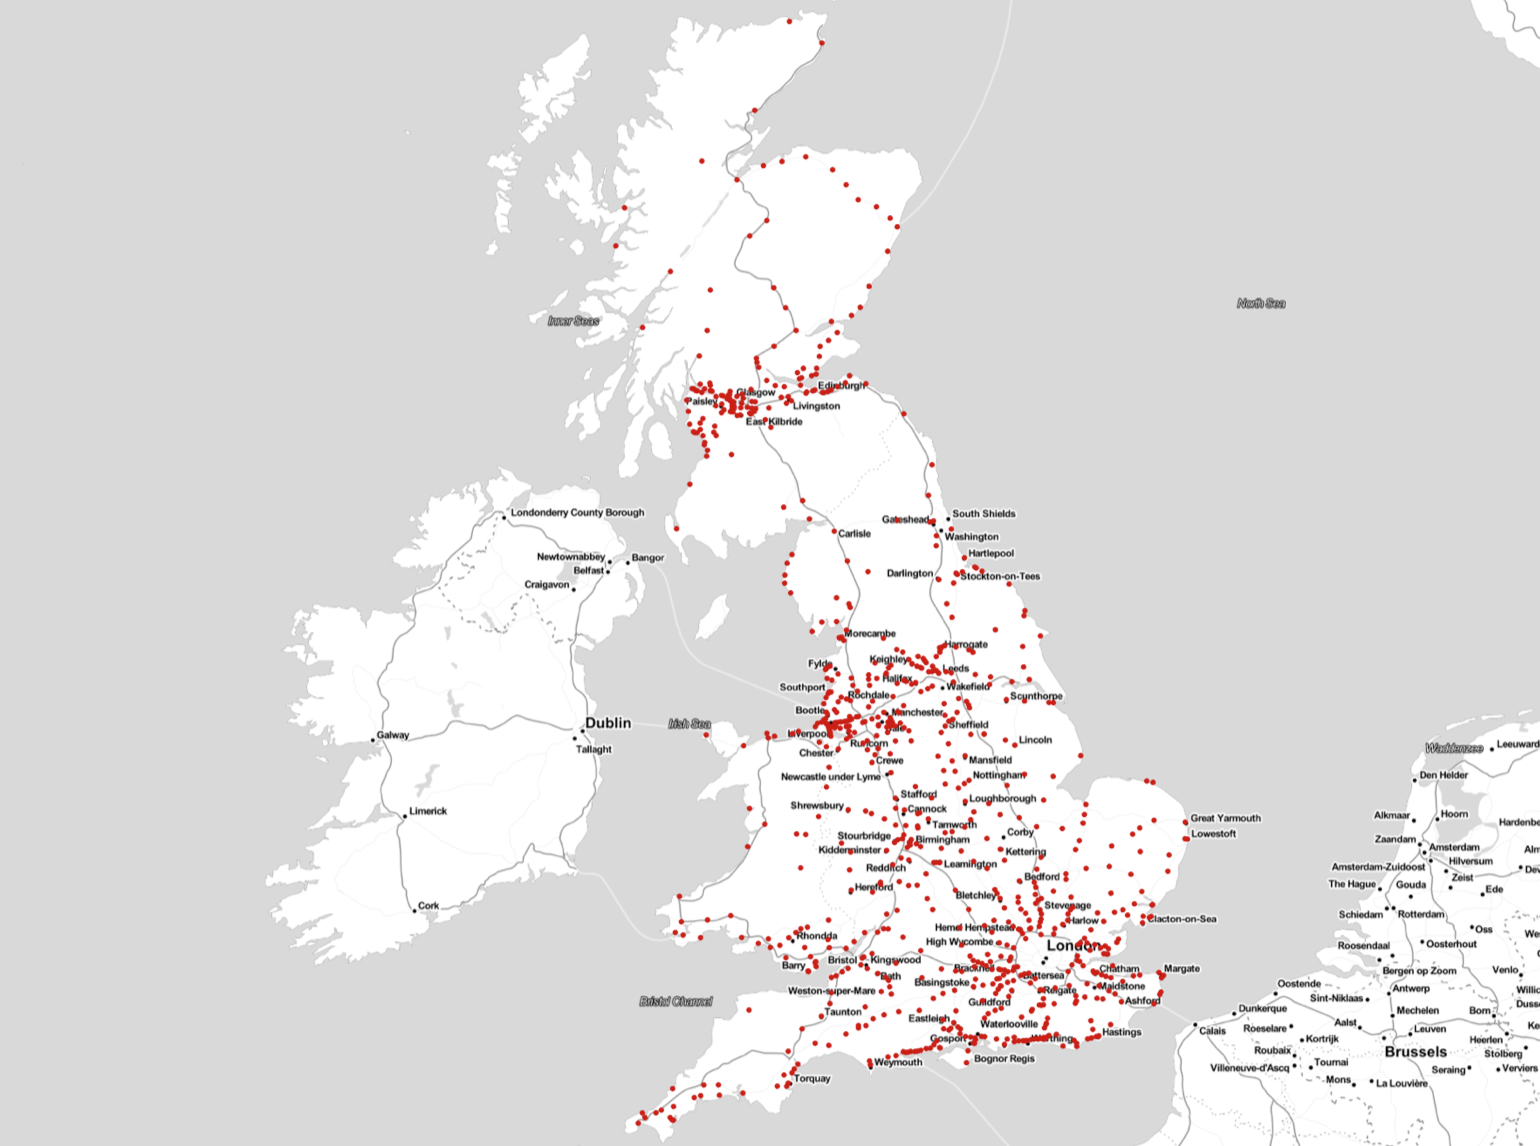
\includegraphics[width=\linewidth]{stations1}
\caption{Stations covered in the 6.184 OD pairs of the RUDD's subset}
\label{fig:stations}
\caption*{Source: Own work}
\end{figure} 

% The dataset also contains information about a set of drivers of demand, but, as discussed in Chapter \ref{chp:lit-rev}, the variables of interest for this study will be restricted to gross value added (GVA) and generalised journey time (GJT), in addition to the volume of journey and revenue variables.

\subsection{Variables}

As discussed in Chapter \ref{chp:lit-rev}, the variables of interest for the current work will be journeys, fares, generalised journey time, and gross added value. This section is dedicated to discuss these variables, what they mean and some particularities about what they actually represent. 

To start it should be highlighted that the variable fares are not directly collected. Instead, it will be approximated by the average revenue per journey. The fact that the main variable in the study is not actually known may represent a vulnerability, nevertheless, it would not be further debated since it is the best information at hand.

Another fact is that, because the dataset is bi-directional, it means that, for example, a trip from Leeds to York and from York to Leeds are identified by the same code, and the variables of journeys and revenues regard both directions summed up. Also, the GVA was collapsed into a single measure that reflects the average GVA of the origin and destination regions. It is, therefore, helpful to consider the OD pair as a connexion, or a route, since the variables will always regard the pair, instead of the location of the origin or the destination by itself. Table \ref{tbl:var_units} summarises information on the variables.


\begin{table}[!ht] \centering 
  \caption{Definition of variables} 
  \label{tbl:var_units} 
{\renewcommand\arraystretch{1.25}}
\begin{tabular} {lllll}
\toprule
Variable          & \multicolumn{2}{m{6cm}}{\raggedright Measure and Unit} & \multicolumn{2}{m{5cm}}{\raggedright Conexion Equivalent Measure} \\
\hline
\textit{Journey}  &\multicolumn{2}{m{6cm}}{\raggedright annual volume of tickets sold, by fare type.} 
				  &\multicolumn{2}{m{5cm}}{\raggedright sum of origin and destina- tion values.}\\
\textit{Fares}    &\multicolumn{2}{m{6cm}}{\raggedright total annual revenue divided by annual volume of tickets sold, by fare type, 2014 values.} 
				  &\multicolumn{2}{m{5cm}}{\raggedright sum of origin and destina- tion values.}\\
\textit{GJT}      &\multicolumn{2}{m{6cm}}{\raggedright sum of journey time, frequency penalty and interchange penalty, as defined in PDFH, in minutes.} 
				  &\multicolumn{2}{m{5cm}}{\raggedright - }\\
\textit{GVA}      &\multicolumn{2}{m{6cm}}{\raggedright regional GVA, at NUTS 3 level, in millions of pounds, 2014 values.} 
				  &\multicolumn{2}{m{5cm}}{\raggedright simple average of origin's and destination's GVA.}\\
\bottomrule
\end{tabular}%
\caption*{Source: Own work}
\end{table} 



\textit{Journeys}

The variable \textit{journeys} is the number of tickets sold per year in each bi-directional route. It does not precisely reflect the number of trips since some tickets allow the passengers to break the journey in a route and make stopovers. Nevertheless, it is a good measure to represent the rail demand. 

To understand the dynamics of this variable Figure \ref{fig:jny} brings two dimensions of journeys: its trend across time and a characterization of journeys by distance.

As shown in Figure \ref{fig:jny_growth_agg} the volume of journeys have consistently increased in the past years. But which kind of journeys are these? Figure \ref{fig:jny_hist} shows that, despite there are very distant routes, as Plymouth to Inverness or Plymouth to Aberdeen, the mass of routes covered by the study peaks around 50 miles and is decrescent as the distance increases. Anyhow, one can affirm that no matter is the class of their length, the aggregate volume of journeys is increasing over the years for all of them, especially for journeys between 100 and 200 miles, as shown by Figure \ref{fig:jny_growth}. 

\begin{figure}[H]
\centering
\begin{subfigure}{\textwidth}
  \centering
  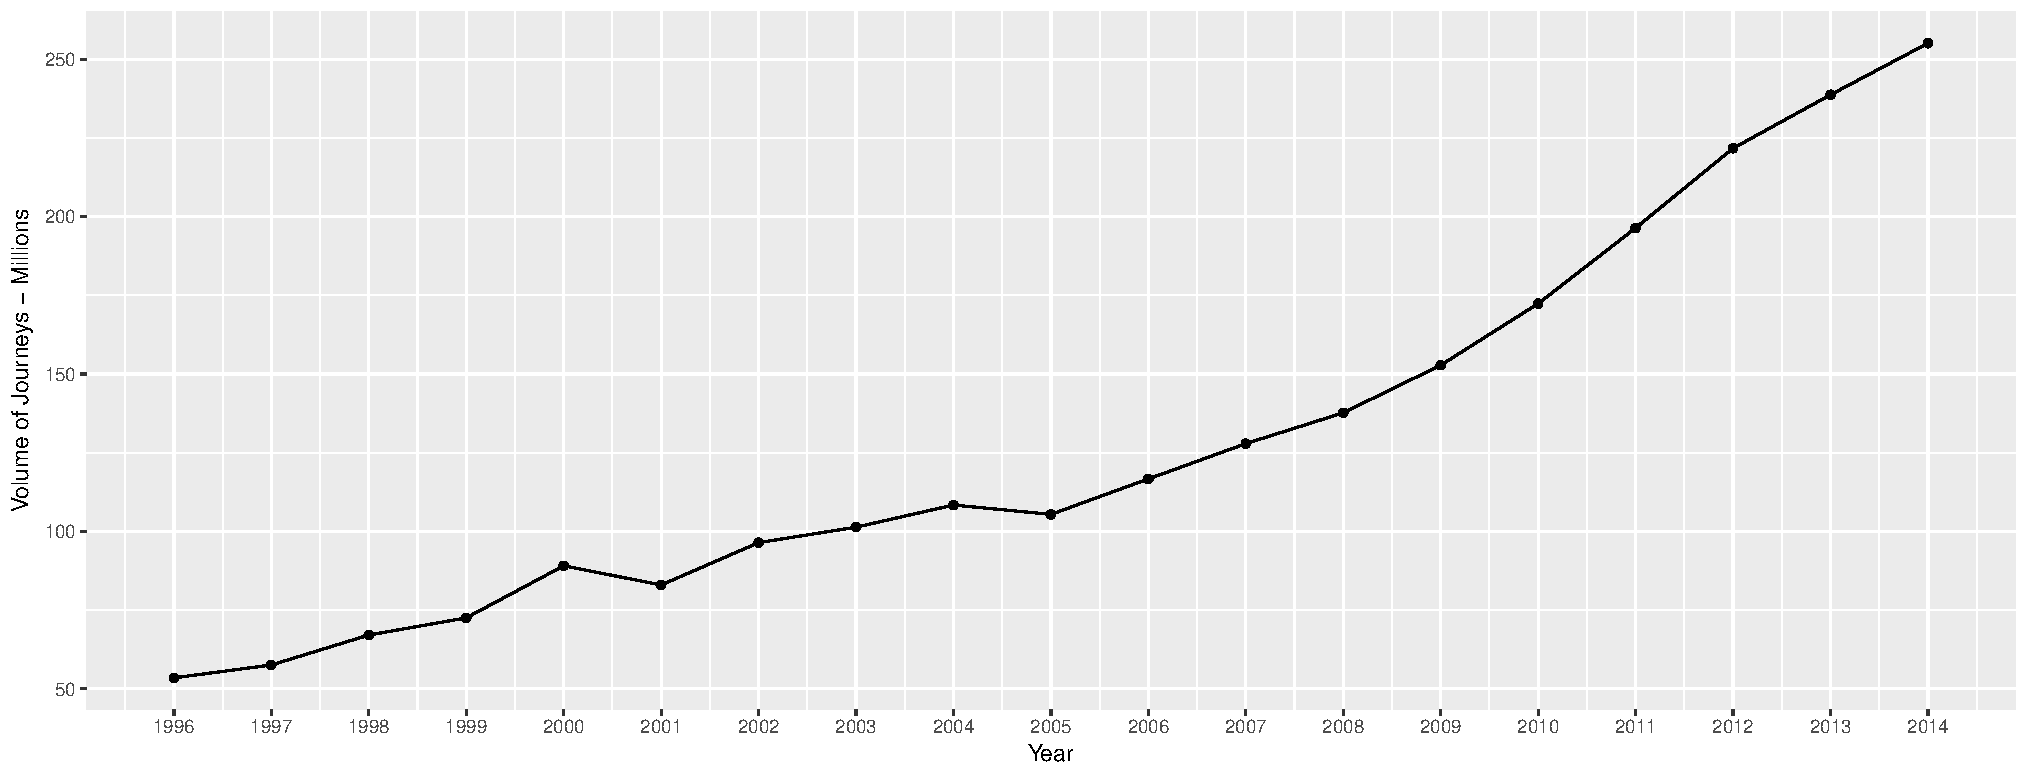
\includegraphics[width=\linewidth]{jny_growth_agg.pdf}
  \caption{Aggregated growth of journeys}
  \label{fig:jny_growth_agg}
\end{subfigure}%

\begin{subfigure}{.5\textwidth}
  \centering
  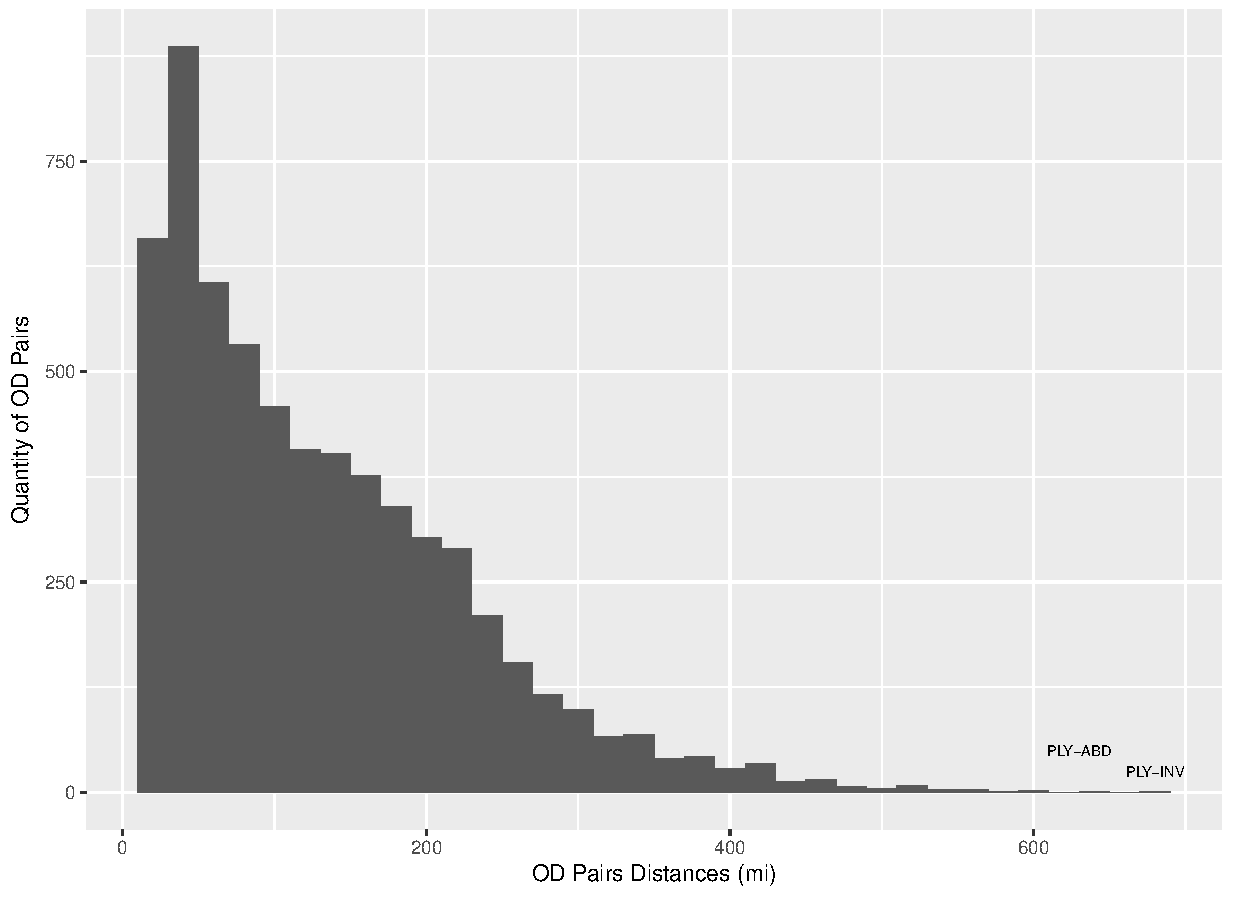
\includegraphics[width=\linewidth]{jny_hist}
  \caption{Distribution of OD pairs' distance}
  \label{fig:jny_hist}
\end{subfigure}%
\begin{subfigure}{.5\textwidth}
  \centering
  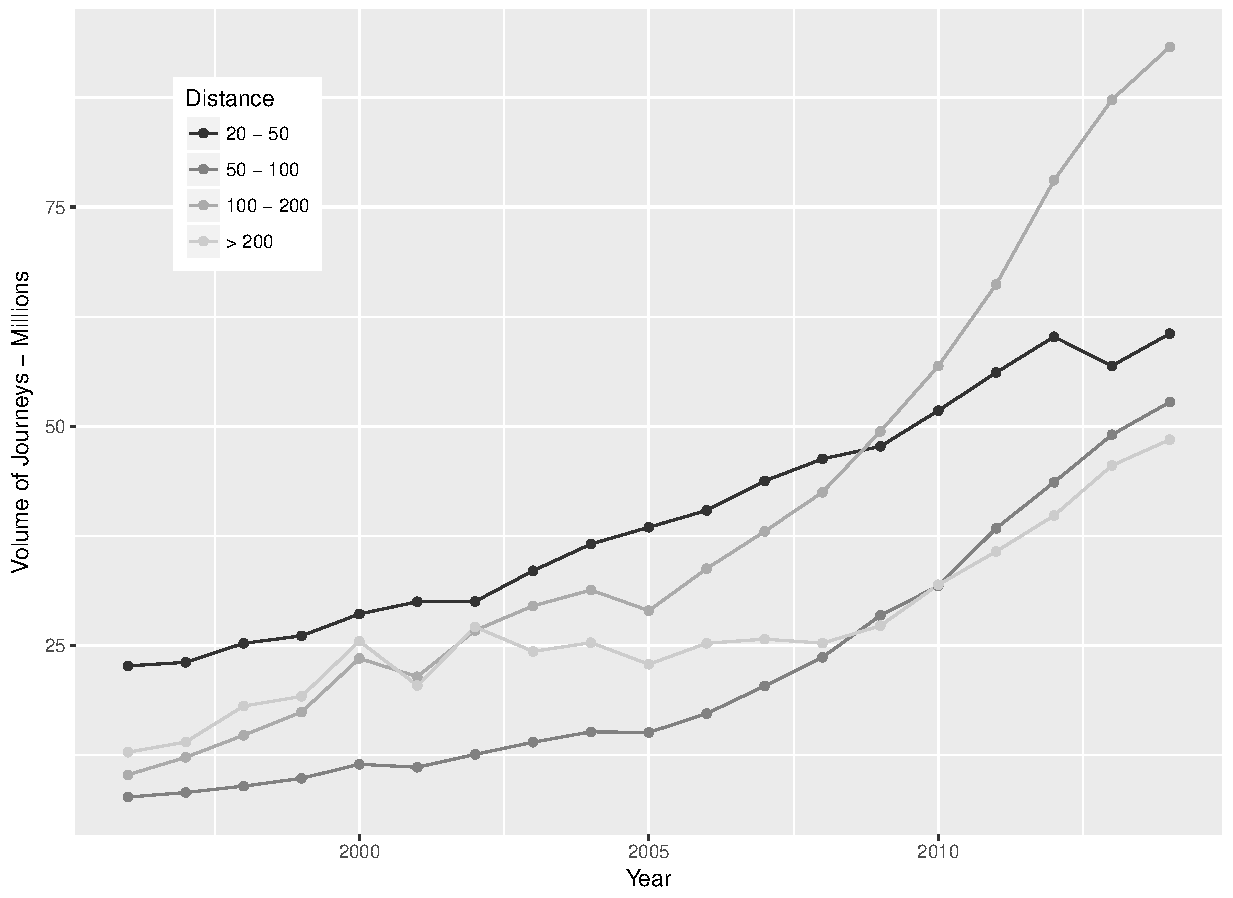
\includegraphics[width=\linewidth]{jny_growth}
  \caption{Growth of journeys per distance class}
  \label{fig:jny_growth}
\end{subfigure}

\caption{Explanatory Analysis on \textit{Journeys}}
\label{fig:jny}
\caption*{Source: Own work}
\end{figure}

\textit{Fares}

In which regards the variable \textit{fares}, Figure \ref{fig:bp_fares} illustrates the range of values in universe of fares for all routes (OD pairs) comprised in the dataset. To make them more comparable they were converted in pounds per mile.

The top row covers the first class fares, separated by type of fare - \textit{full}, \textit{reduced} and \textit{advance}. The bottow row refers to the standard class.

From these graphs one may notice that the range of \textit{full} fares is increasing over the time, both for first and standard class. The \textit{reduced} fare, in turn, shows a significantly smaller range in the standard class, whilst for the first class, it does not seem to follow a pattern. The restricted range of the standard reduced fares may be due to the ceiling imposed by regulation, as discussed in Chapter \ref{chp:lit-rev}.

Lastly, in which regards the \textit{advance} fares, which is a mix of discounted \textit{full} and \textit{reduced}, they present a steady median, slightly slower than the reduced fares but with a wider range in the standard class. For the first class, despite the lack o pattern for the \textit{reduced} fare, the advance also shows a steady median, lower than the \textit{full}, with a step change in the year 2000, which was also observed in the \textit{reduced}. 

\begin{figure}[H]
\centering
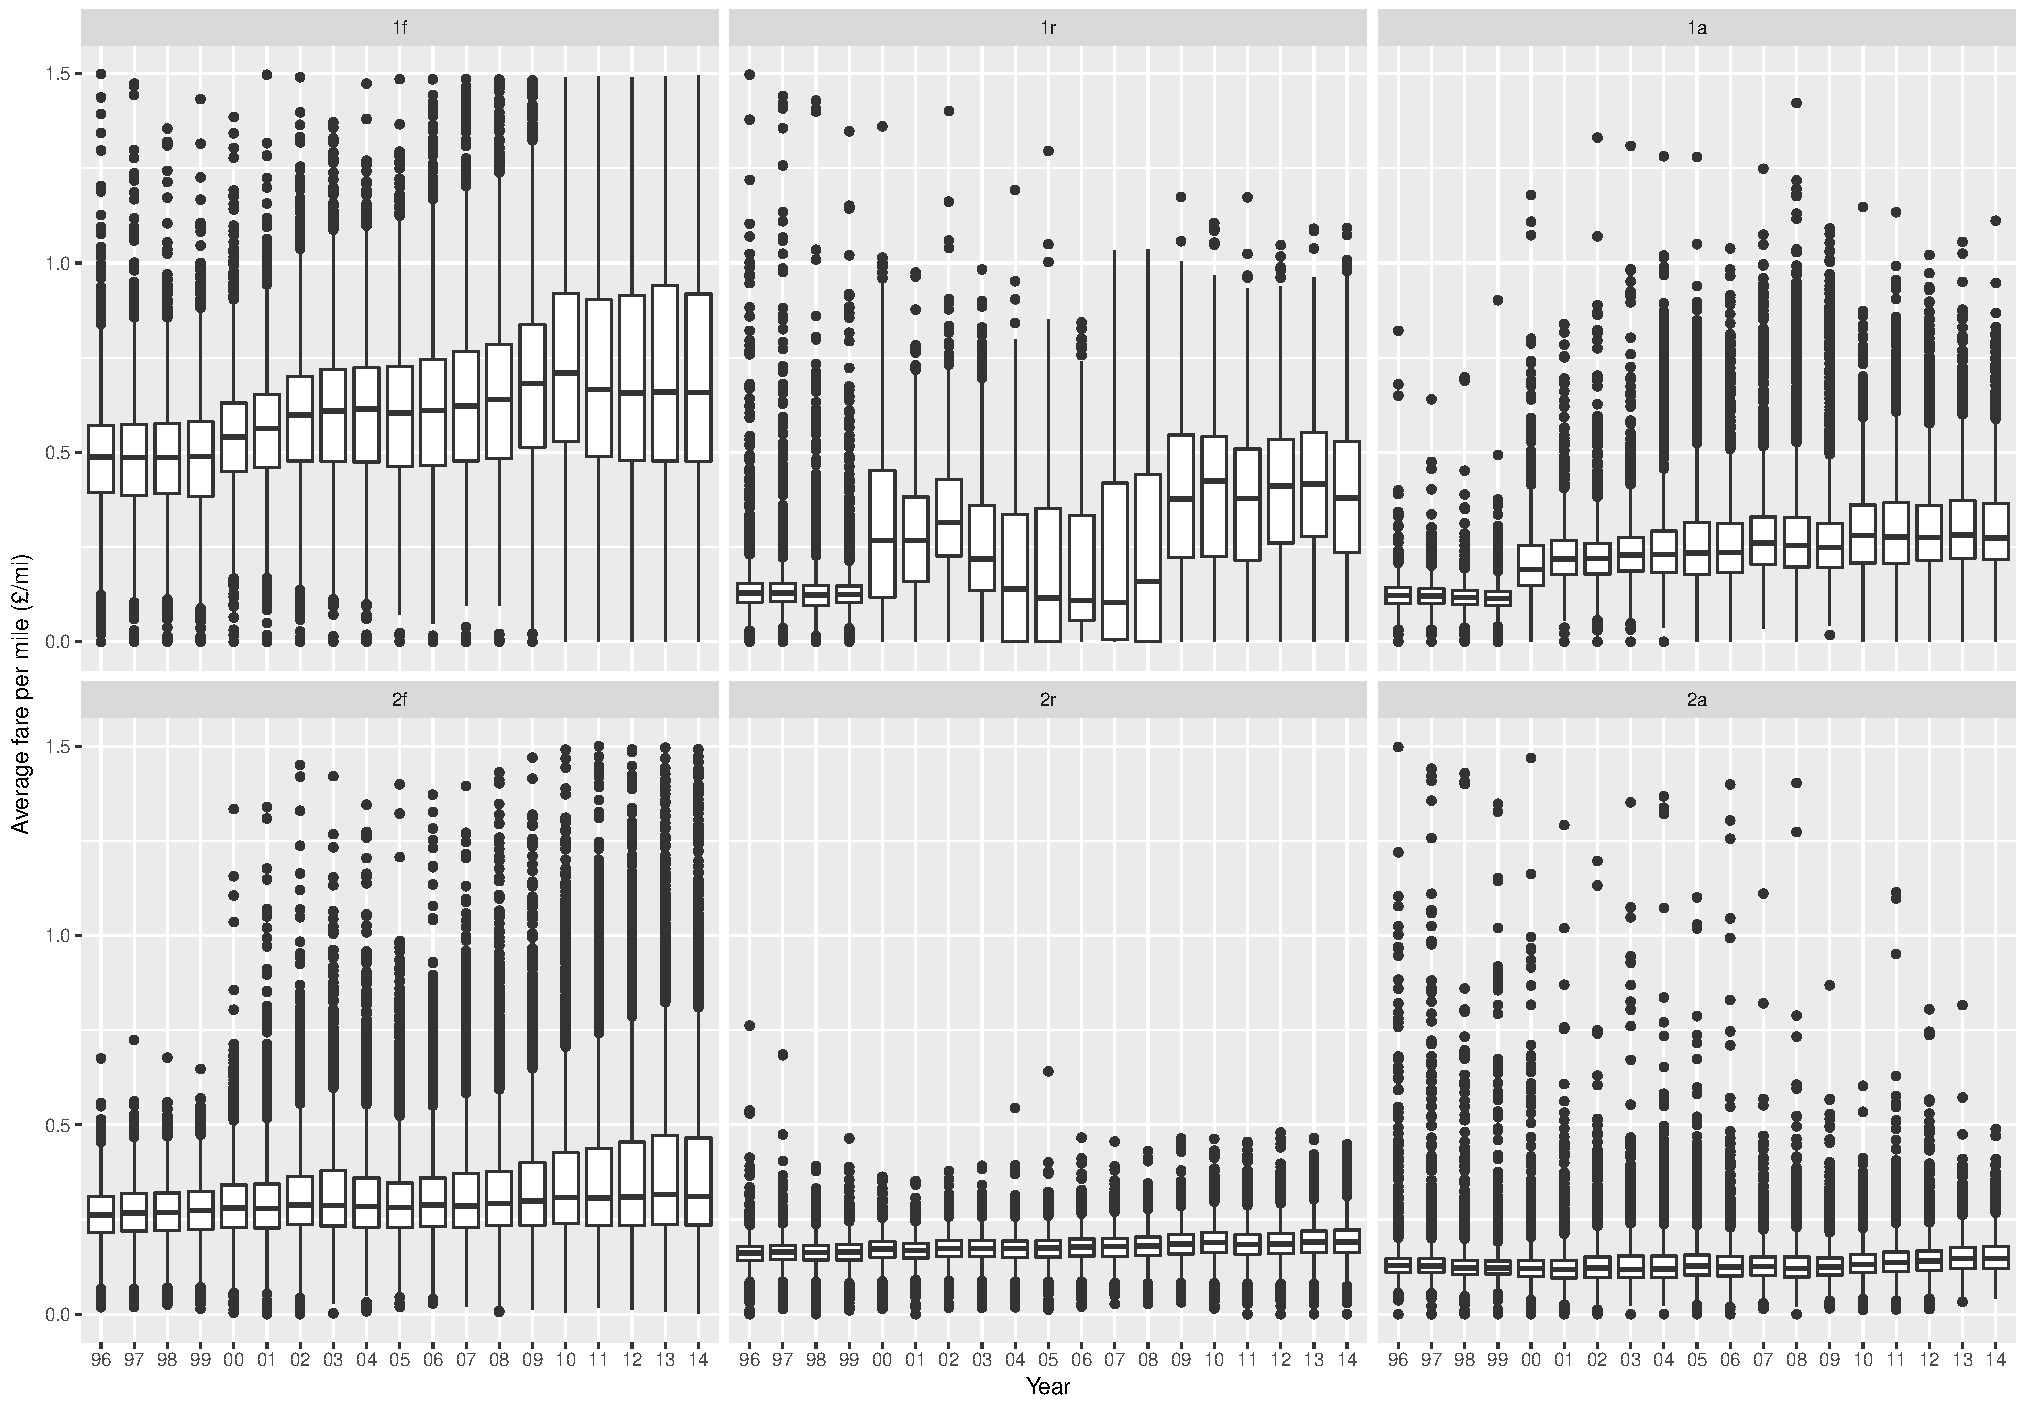
\includegraphics[width=\linewidth]{bp_fares}
\caption{Dispersion of fares per mile accross the OD pairs}
\label{fig:bp_fares}
\caption*{Source: Own work}
\end{figure} 

\textit{Gross Added Value - GVA}

The GVA is a metric for the level of economic activity in a given region. Because rail demand is expected to have a positive polarity with economic activity \citep{pdfh} - the higher GVA, the higher volume of journeys - it is interesting to check this dynamic on the data.

To visualise it, the variable GVA was segmented in four levels. For each level, the average volume of journeys was calculated per year. As shown in Figure \ref{fig:gva_jny}, the higher the GVA level, the higher the average volume of journeys per route. Also, it is possible to notice an overall trend of growth of journeys for all levels of GVA. 

To complement the visualization, Figure \ref{fig:gva_od} brings more information about the range of GVA among the ODs pairs and how was the dynamic across the years. Because the OD pairs in the dataset remained constant over the years, with very few exceptions, one can notice that, in general terms, there was a trend towards the right. That means that regions are escalating to levels of higher economic activity. 

For the lowest level of GVA, at the left, it seems that have occurred a concentration movement which peaks very close to the boundary of the next level. Eventually, these OD pairs may have changed to next level of GVA. Also, the second and third levels seem to have spread towards the right. Lastly, the highest level of GVA appeared only in the year 2000 and seems to have a mild movement of expansion and contraction.

\begin{figure}[H]
\centering
\begin{subfigure}{.5\textwidth}
  \centering
  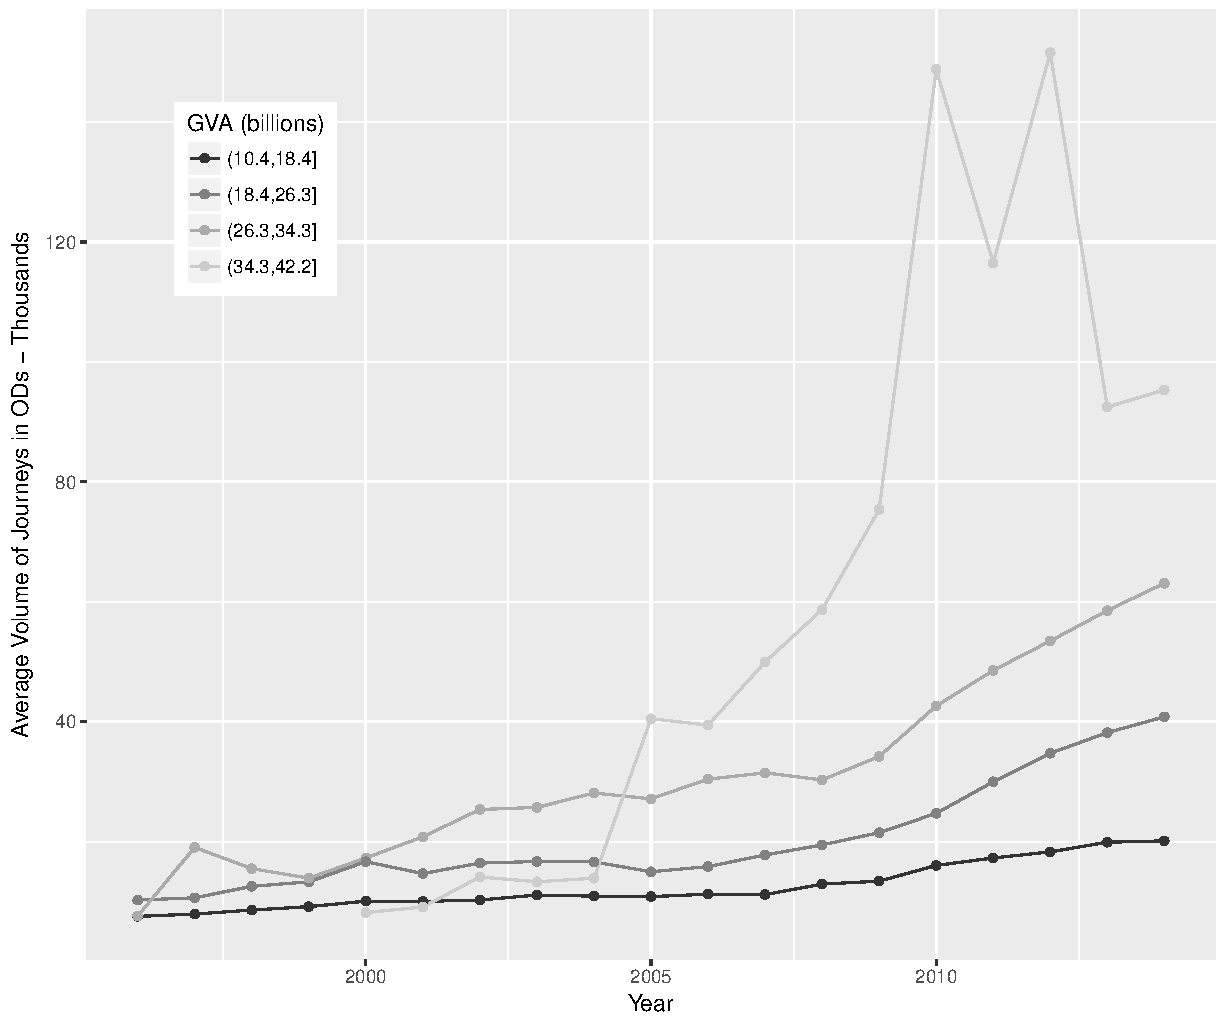
\includegraphics[width=\linewidth]{gva_jny}
  \caption{Growth journeys by level of GVA}
  \label{fig:gva_jny}
\end{subfigure}%
\begin{subfigure}{.5\textwidth}
  \centering
  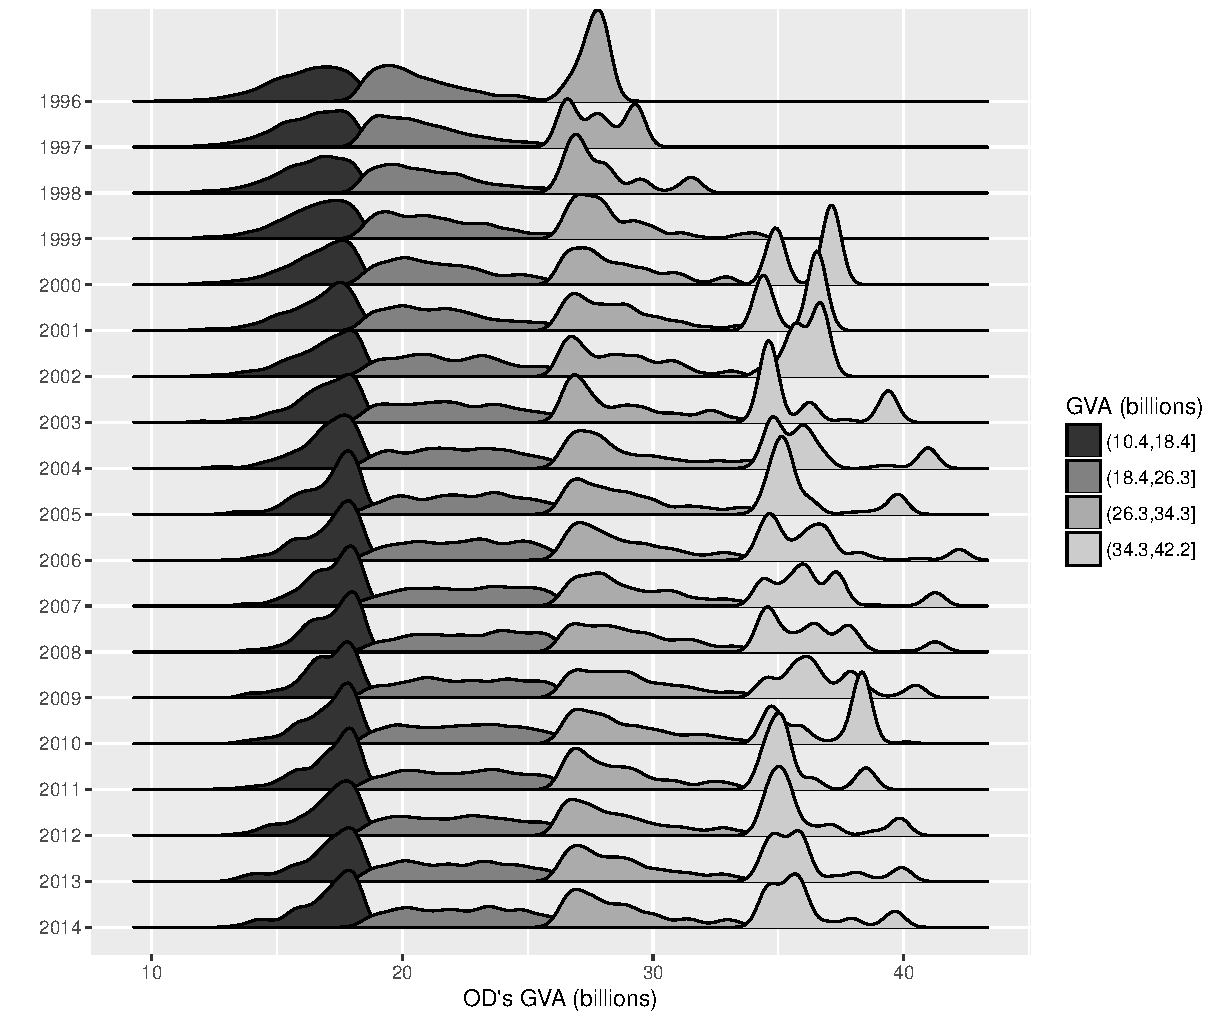
\includegraphics[width=\linewidth]{gva_od}
  \caption{Distribution of OD pairs' GVA}
  \label{fig:gva_od}
\end{subfigure}%
\caption{Exploratory Analysis on \textit{GVA}}
\label{fig:gva}
\caption*{Source: Own work}
\end{figure}

In short, eyeballing the \textit{GVA} variable it is possible to identify consistency between the theoretical relation of economic activity and rail journeys in the data.
\\[3pt]

% \begin{figure}[H]
% \centering
% \begin{subfigure}{.5\textwidth}
%   \centering
%   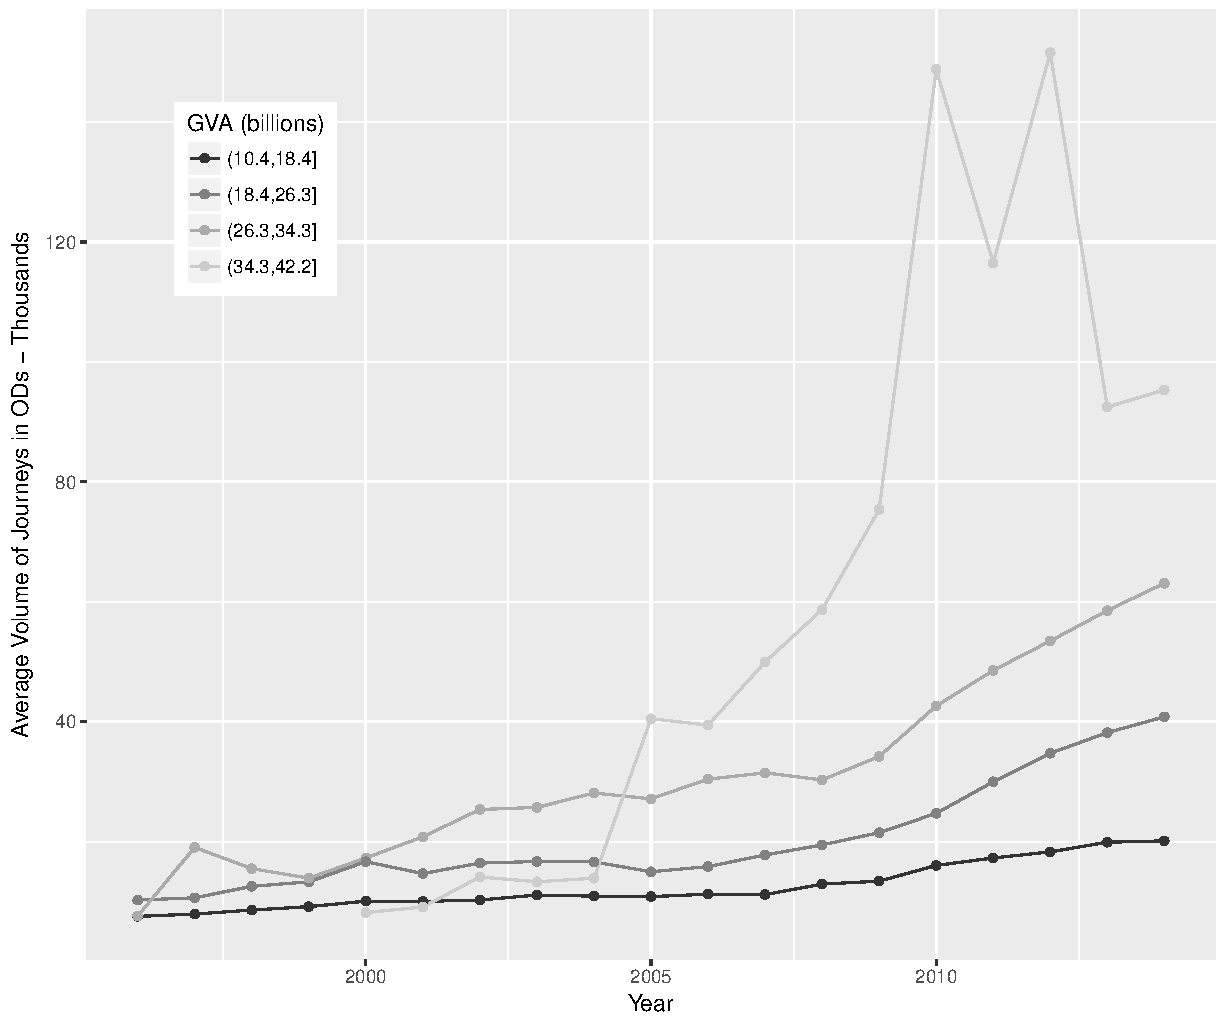
\includegraphics[width=\linewidth]{gva_jny}
%   \caption{Growth journeys by level of GVA}
%   \label{fig:gva_jny}
% \end{subfigure}%
% \begin{subfigure}{.4\textwidth}
%   \centering
%   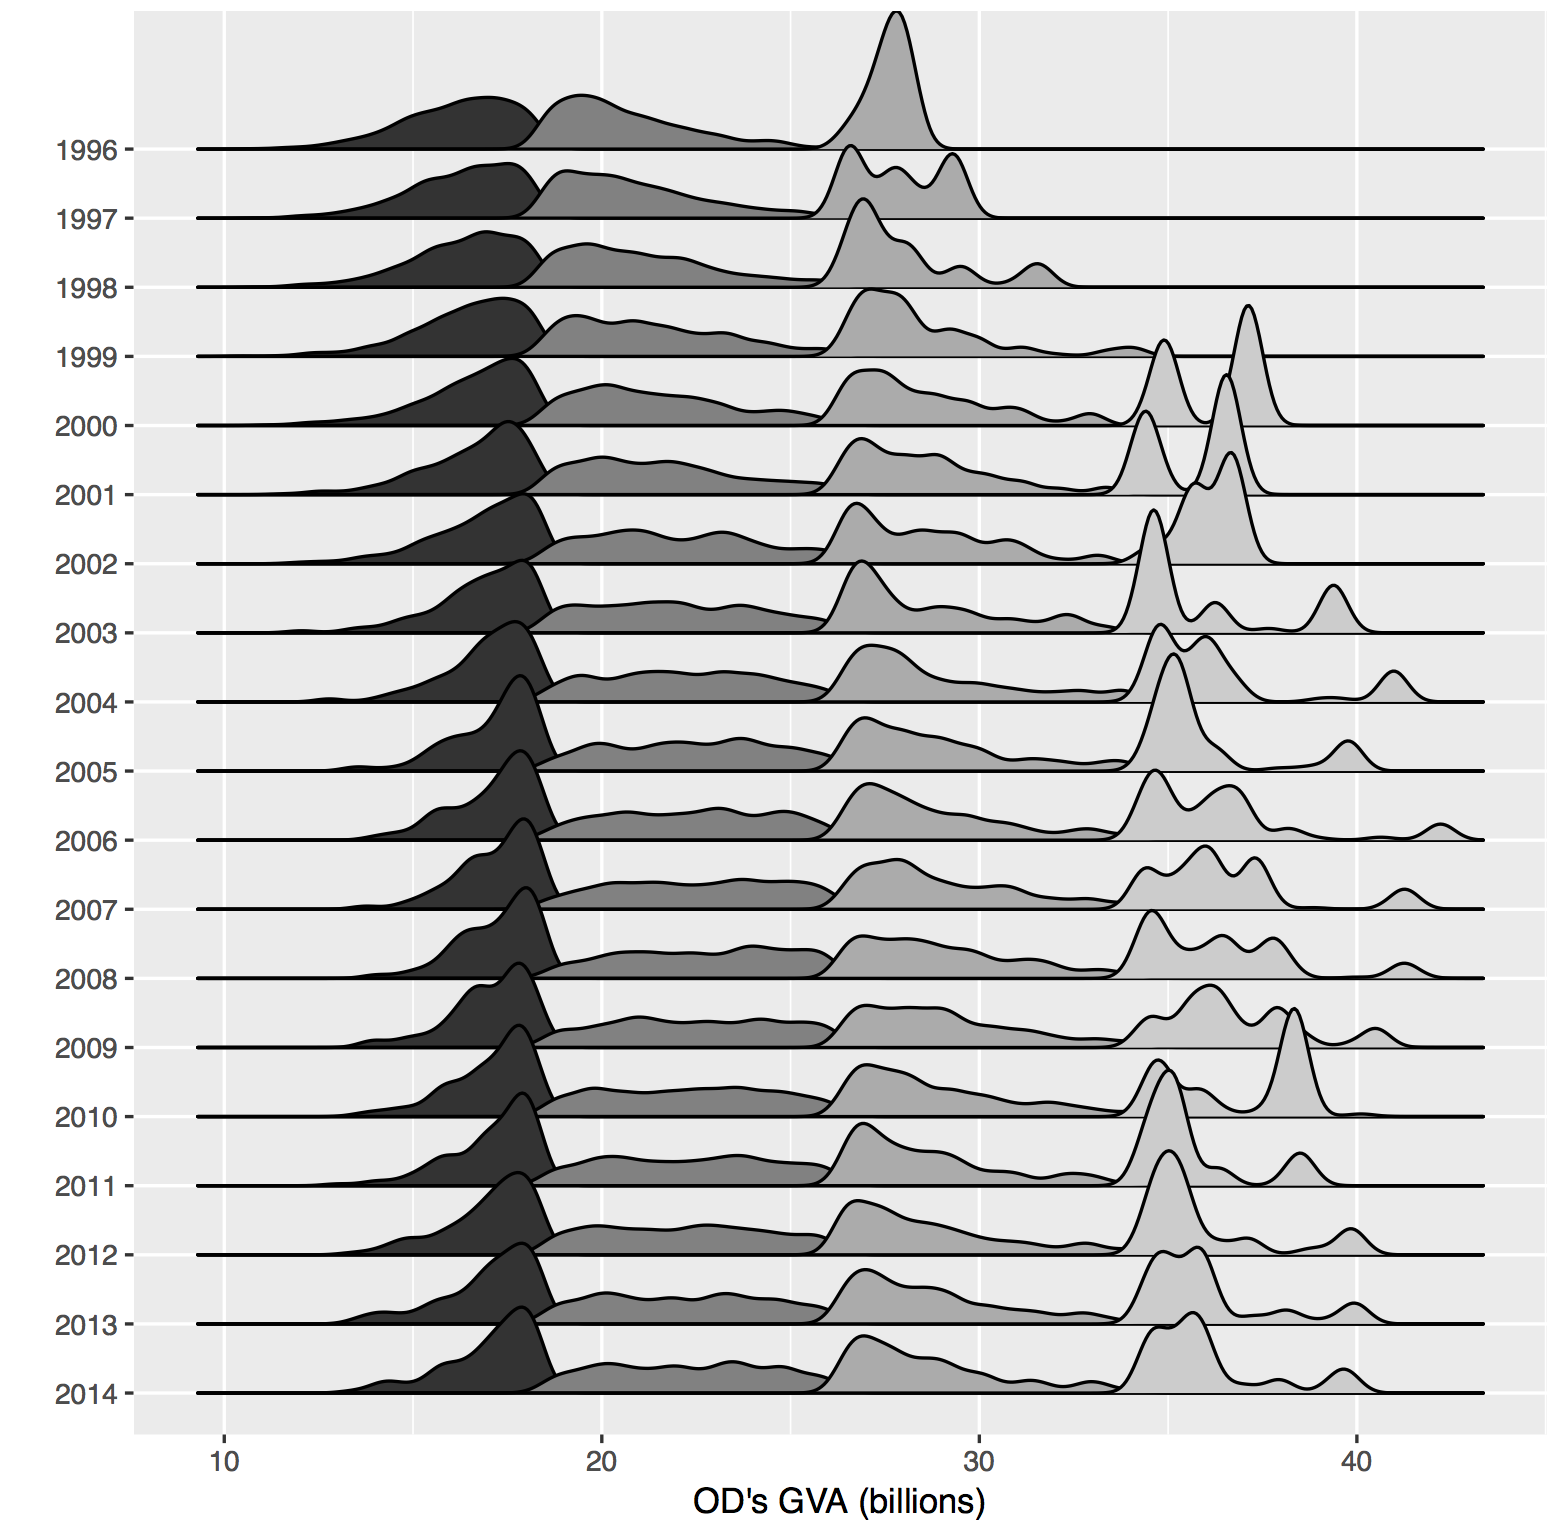
\includegraphics[width=\linewidth]{gva_od1}
%   \caption{Distribution of OD pairs' GVA}
%   \label{fig:gva_od}
% \end{subfigure}%
% \begin{subfigure}{.2\textwidth}
%   \centering
%   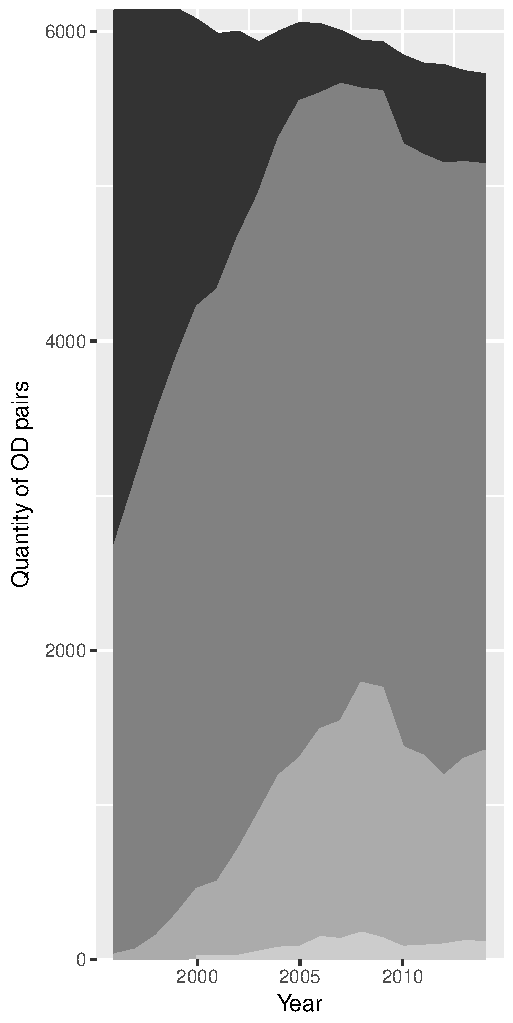
\includegraphics[width=\linewidth]{od}
%   \caption{OD pairs by GVA}
%   \label{fig:d}
% \end{subfigure}%
% \caption{Explanatory Analysis on \textit{GVA}}
% \label{fig:gva}
% \caption*{Source: Own elaboration}
% \end{figure}


\textit{Generalised Journey Time - GJT}

In this work, the GJT measure represents the quality-related drivers of demand. It comprises the journey time plus the frequency and interchange penalties, as defined in PDFH, and it is measured in minutes.

To understand the dynamics of this variable Figure \ref{fig:gjt} brings two dimensions of it: an overview of the GJT of the OD pairs considered in the study and the accumulated average reduction of GJT over the years, taking the year 1996 as the base.

Figure \ref{fig:gjt_hist} shows the overall distribution of routes by GJT. As a general characterization, it is possible to observe that the mass of routes peaks around 150 minutes and decreases as the GJT increases, achieving extreme values over 1,000 minutes. 

Additionally, Figure \ref{fig:gjt_years} shows how, in average, routes are reducing their GJT over the years. The values plotted in the graph are accumulated reductions with respect to the year 1996. It is observed an average reduction of 7.3\% in the GJT in 19 years (1996-2014).

\begin{figure}[H]
\centering
\begin{subfigure}{.5\textwidth}
  \centering
  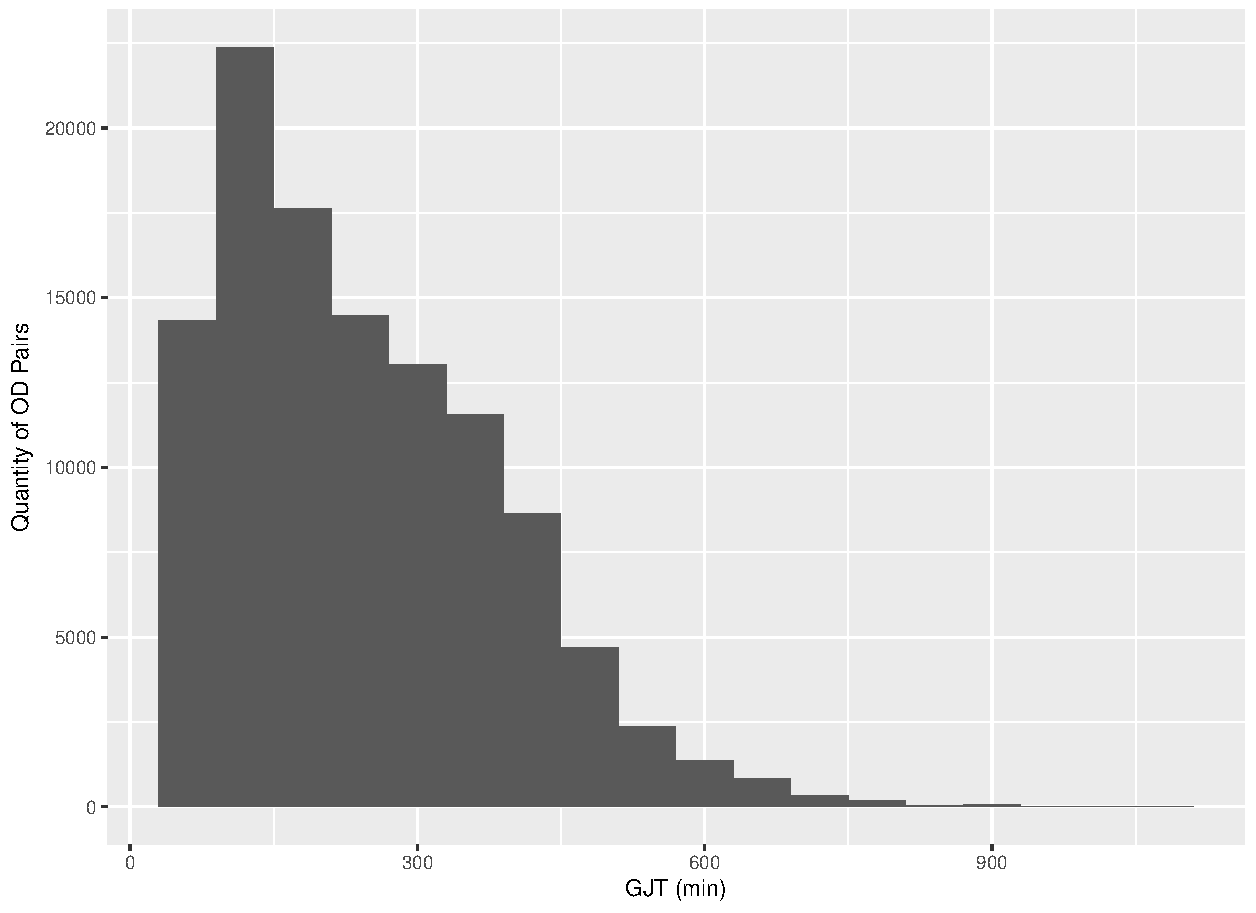
\includegraphics[width=\linewidth]{gjt_hist}
  \caption{Distribution of GJT across the routes}
  \label{fig:gjt_hist}
\end{subfigure}%
\begin{subfigure}{.5\textwidth}
  \centering
  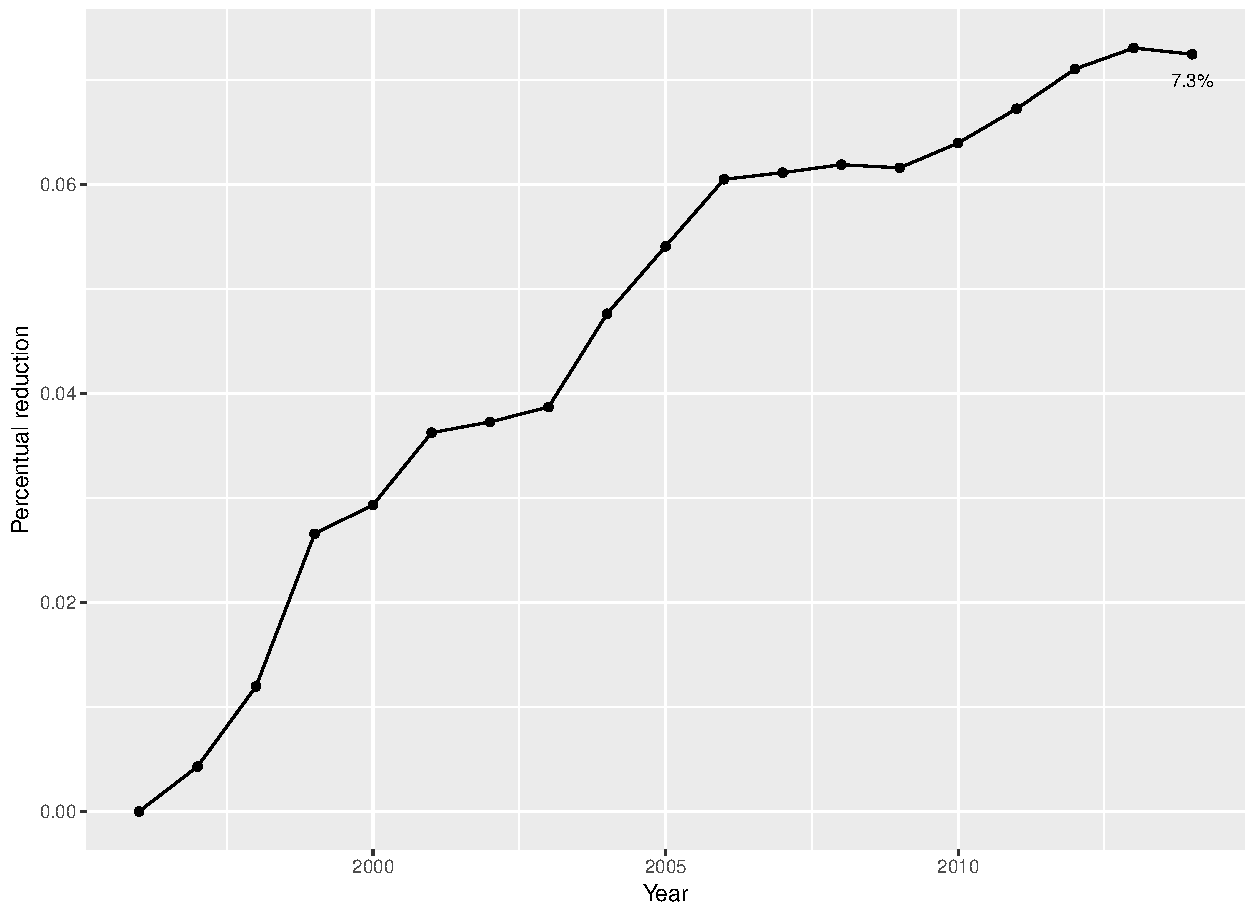
\includegraphics[width=\linewidth]{gjt_years}
  \caption{Accumulated Reduction of GJT}
  \label{fig:gjt_years}
\end{subfigure}%
\caption{Exploratory Analysis on \textit{GJT}}
\label{fig:gjt}
\caption*{Source: Own work}
\end{figure}

\subsection{Subsetting markets in the dataset}

The availability or not of a different set of tickets across the routes creates different markets environments. When there are more types of fares the competition increases and the market share of tickets is affected simply because there are more options at one's disposal. 

% For instance, a big player is the first class tickets.

Therefore, the existence of different sets of fares in a route affects the fare elasticities. For example, the fare elasticity of reduced tickets with respect to the demand for full tickets may differ whether there is or not the first class ticket.

The dataset was subsetted into four markets to properly estimate the fare elasticities for each circumstance. The two first will regard only the standard class, and in the other two, first class will be added. 

With the introduction of first class tickets in the Markets 3 and 4, their complexity has increased significantly. To overcome that, the coverage of the dataset was shortened to a regional level to reduce the unobserved heterogeneity and provide a more well-behaved data. The regions \footnote{NUTS 1 level regions.} chosen were Scotland and Yorkshire and Humber, so only routes which both origin and destination in these regions were considered. There was no strong justification for choosing these regions beyond the fact that any interference with London flows was avoided.

An alternative to keep the broad coverage and reduce the heterogeneity that may exist across regions could be the adoption of dummy variables to capture these unobserved characteristics. However, this option was not adopted because in the Bayesian framework it would represent an increase of 10 marginal posterior distributions (from the 11 regions), in each regression model. It was considered, thus, that such complexity was needless since this is an introductory study of Bayesian econometrics in the field. It is important to be aware, however, that a cut in the dataset is a stronger isolation of unobserved characteristics than regressing with dummy variables. 

Table \ref{tbl:market_subs} presents summary information on the resultant dataset for each market.


\begin{table}[H] \centering 
  \caption{Market subsetting} 
  \label{tbl:market_subs} 
{\renewcommand\arraystretch{1.25}}
\begin{tabular} {cccccc}
\toprule
Market             & Fares      & OD Pairs & Time Series & Obs  & Coverage\\
\hline
1                  & 2F, 2R         & 2,074     & 1996 - 2014   & 15,481 & Great Britain\\
\hline
2                  & 2F, 2R, 2A     & 1,550     & 2000 - 2014 & 5,909  & Great Britain\\
\hline
\multirow{2}{*}{3} & 1N, 2F, 2R,  & \multirow{2}{*}{516} & \multirow{2}{*}{1996 - 2014} & \multirow{2}{*}{5,783} & Scotland - Yorkshire \\
                   &   2A         &                      &                              &                        & and Humber\\
\hline
\multirow{2}{*}{4} & 1F, 1R, 1A,& \multirow{2}{*}{251} & \multirow{2}{*}{1996 - 2014} & \multirow{2}{*}{1,738} & Scotland - Yorkshire \\ 
				   & 2F, 2R, 2A &                        &                              &                      & and Humber\\
\bottomrule
\end{tabular}%
\caption*{Source: Own work}
\end{table} 



It should not be expected, however, that the quantity of OD pairs shown in Table \ref{tbl:market_subs} to be constant over the years because the availability of tickets for a given route is not fixed in time. It may happen that the quantity of ODs pairs in each market varies from year to year. For example, if in a given route the first class ticket started being commercialised in the year 2000 onwards, this OD pair was considered in market 1 or 2 before 2000 and in market 3 or 4 after that. The important is that the pool of each market is coherent with their actual competition conditions. For completeness, Figure \ref{fig:od_mkts} illustrates the variation of OD pairs in each market.

\begin{figure}[H]
\centering
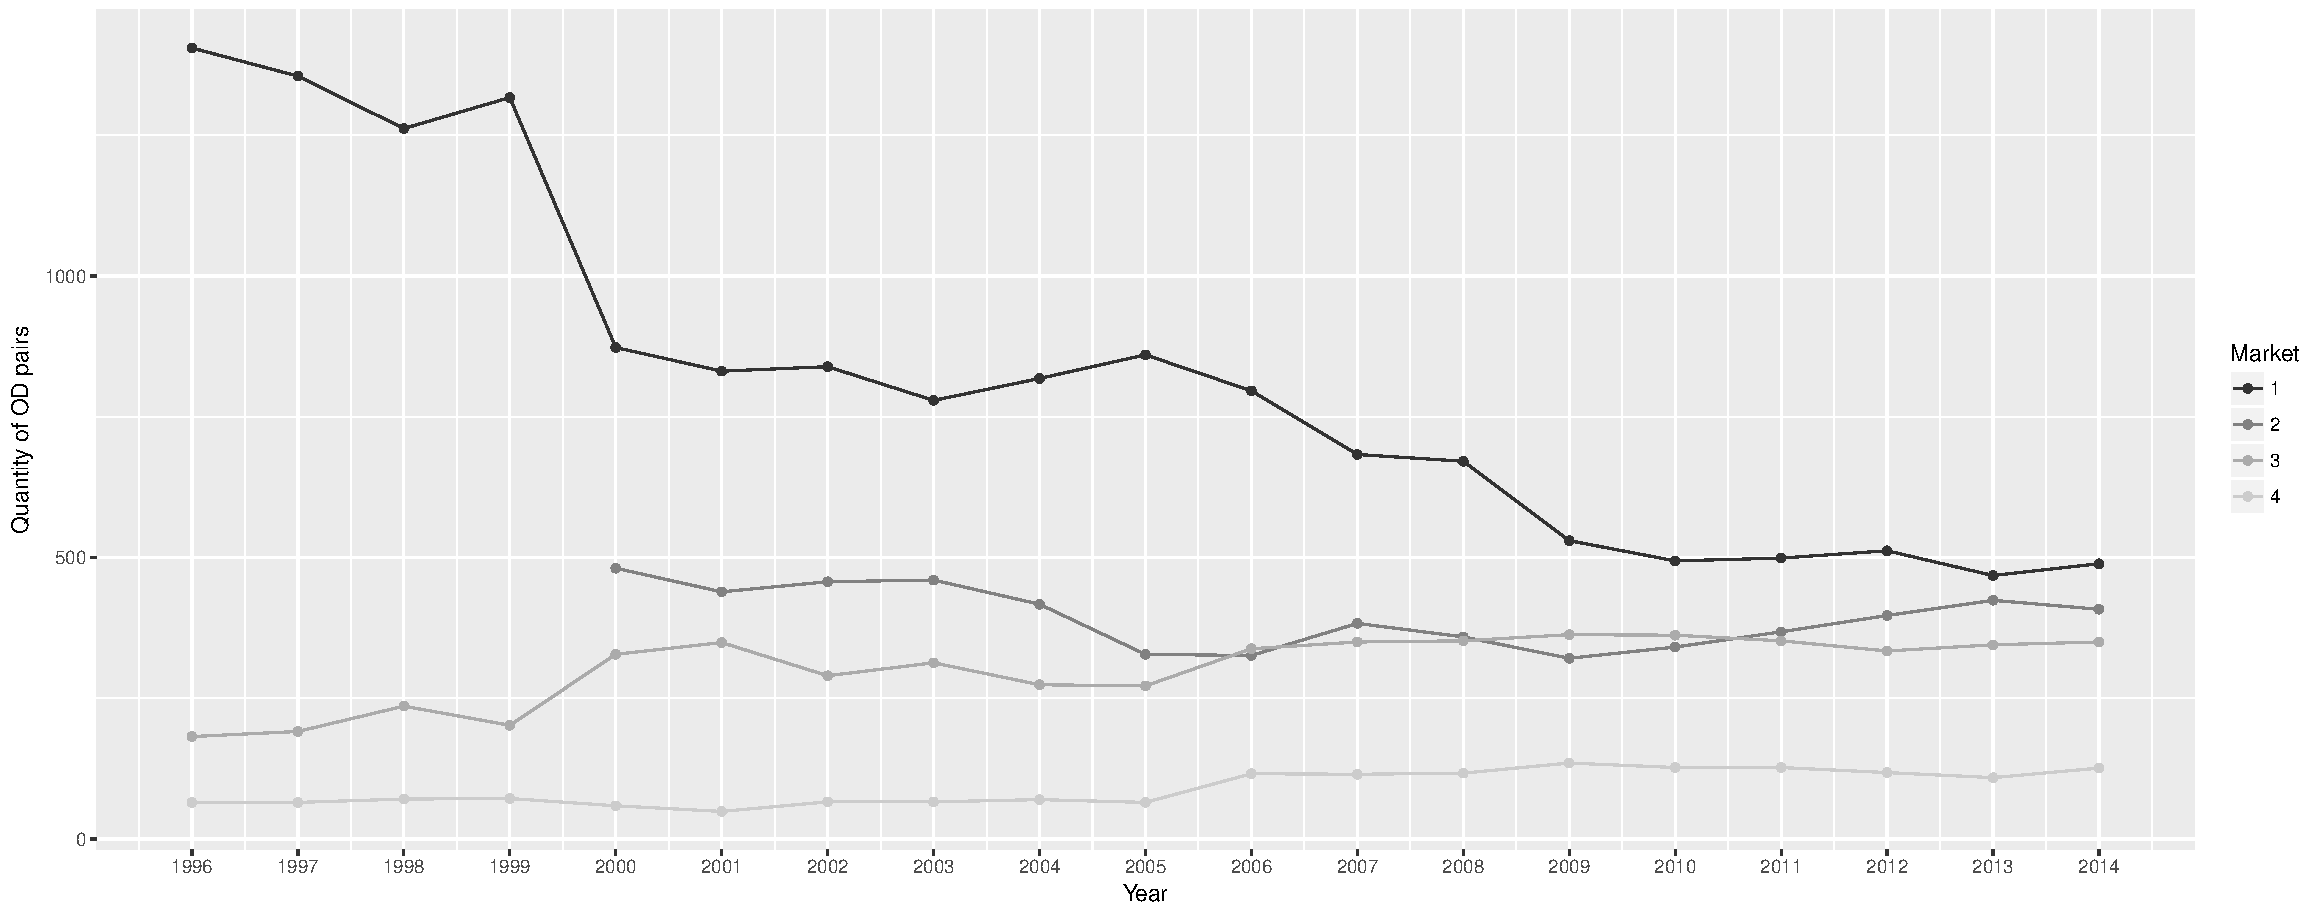
\includegraphics[width=\linewidth]{od_mkt.pdf}
\caption{Quantity of OD pairs by market along the years}
\label{fig:od_mkts}
\caption*{Source: Own work}
\end{figure} 

Another aspect that may be relevant to analyse the results is the market share of fares. Table \ref{tbl:mktshr} shows these numbers.

It is noticeable that in all markets the dominance of the \textit{standard reduced} fare, followed by the \textit{standard full}. It is also noticeable that the \textit{advance} ticket has been gaining space, growing from 1\% to 8\% in 15 years, in Market 2, and from 4\% to 12\% in Market 3. The \textit{first class} tickets presented a small market share, in decline in both Markets 3 and 4, from 7\% to 3\% and 5-6\% to 2-0\%, respectively. It is observable that the \textit{First Class} tickets when disaggregated by fare type show very small market shares, even less than 1\%.

\begin{landscape}

\begin{table}[!ht] \centering 
  \caption{Market share of fares by market segmentation} 
  \label{tbl:mktshr} 
{\renewcommand\arraystretch{1.25}}
\begin{tabular} {cccccccccccccccccccc}
  \toprule
  &\multicolumn{2}{c}{Market 1} & & \multicolumn{3}{c}{Market 2} & & \multicolumn{4}{c}{Market 3} & & \multicolumn{6}{c}{Market 4} \\
 \cline{2-3} \cline{5-7} \cline{9-12} \cline{14-19} 
 Year & 2F  & 2R   & & 2F   & 2R   & 2A  & & 1N  & 2F   & 2R   & 2A   & & 1F & 1R & 1A & 2F & 2R & 2A \\ 
  \hline
1996 & 41\% & 59\% & & -    & -    & -   & & 7\% & 28\% & 61\% & 4\%  & & 5\% & 5\% & 6\% & 7\%  & 66\% & 11\% \\ 
1997 & 39\% & 61\% & & -    & -    & -   & & 7\% & 32\% & 55\% & 6\%  & & 4\% & 9\% & 6\% & 7\%  & 60\% & 15\% \\ 
1998 & 38\% & 62\% & & -    & -    & -   & & 7\% & 31\% & 57\% & 5\%  & & 4\% & 8\% & 5\% & 12\% & 58\% & 13\% \\ 
1999 & 37\% & 63\% & & -    & -    & -   & & 9\% & 26\% & 58\% & 7\%  & & 5\% & 8\% & 6\% & 7\%  & 59\% & 15\% \\ 
2000 & 39\% & 61\% & & 26\% & 73\% & 1\% & & 2\% & 34\% & 58\% & 6\%  & & 4\% & 0\% & 0\% & 26\% & 58\% & 11\% \\ 
2001 & 38\% & 62\% & & 31\% & 68\% & 1\% & & 2\% & 34\% & 59\% & 5\%  & & 4\% & 0\% & 0\% & 27\% & 60\% &  8\% \\ 
2002 & 39\% & 61\% & & 25\% & 73\% & 2\% & & 3\% & 32\% & 59\% & 6\%  & & 4\% & 0\% & 0\% & 26\% & 60\% & 10\% \\ 
2003 & 38\% & 62\% & & 33\% & 66\% & 1\% & & 2\% & 28\% & 64\% & 6\%  & & 3\% & 0\% & 0\% & 21\% & 65\% & 10\% \\ 
2004 & 39\% & 61\% & & 32\% & 67\% & 1\% & & 3\% & 26\% & 64\% & 8\%  & & 3\% & 0\% & 1\% & 17\% & 68\% & 11\% \\ 
2005 & 38\% & 62\% & & 32\% & 66\% & 2\% & & 2\% & 25\% & 67\% & 6\%  & & 3\% & 0\% & 1\% & 17\% & 68\% & 11\% \\ 
2006 & 38\% & 62\% & & 35\% & 62\% & 2\% & & 2\% & 27\% & 64\% & 6\%  & & 3\% & 0\% & 1\% & 21\% & 65\% & 11\% \\ 
2007 & 38\% & 62\% & & 38\% & 60\% & 2\% & & 2\% & 31\% & 62\% & 5\%  & & 3\% & 0\% & 1\% & 23\% & 61\% & 11\% \\ 
2008 & 39\% & 61\% & & 36\% & 61\% & 3\% & & 3\% & 31\% & 62\% & 4\%  & & 3\% & 0\% & 1\% & 26\% & 62\% &  8\% \\ 
2009 & 43\% & 57\% & & 38\% & 59\% & 3\% & & 3\% & 29\% & 59\% & 8\%  & & 3\% & 2\% & 1\% & 25\% & 57\% & 12\% \\ 
2010 & 43\% & 57\% & & 38\% & 58\% & 4\% & & 3\% & 26\% & 63\% & 8\%  & & 2\% & 1\% & 1\% & 20\% & 64\% & 12\% \\ 
2011 & 45\% & 55\% & & 40\% & 56\% & 4\% & & 3\% & 26\% & 62\% & 9\%  & & 1\% & 1\% & 1\% & 20\% & 63\% & 13\% \\ 
2012 & 47\% & 53\% & & 38\% & 56\% & 6\% & & 3\% & 23\% & 65\% & 9\%  & & 1\% & 1\% & 1\% & 16\% & 68\% & 12\% \\ 
2013 & 46\% & 54\% & & 35\% & 58\% & 6\% & & 3\% & 31\% & 55\% & 12\% & & 2\% & 0\% & 2\% & 28\% & 49\% & 19\% \\ 
2014 & 43\% & 57\% & & 37\% & 55\% & 8\% & & 3\% & 33\% & 52\% & 12\% & & 2\% & 0\% & 2\% & 28\% & 48\% & 20\% \\
   \bottomrule
\end{tabular}
\caption*{Source: Own work}
\end{table}

\end{landscape}

\subsection{Data correlation}

As mentioned in Chapter \ref{chp:lit-rev}, the correlation has been a problem in the previous studies in fares elasticities estimation.

Checking the data used in this study, it is noticed that correlation is also present, as should be expected. Figure \ref{fig:cor} presents correlation matrixes of the fares variables for each market after the segmentation of the dataset.

\begin{figure}[H]
\centering
\begin{subfigure}{.5\textwidth}
  \centering
  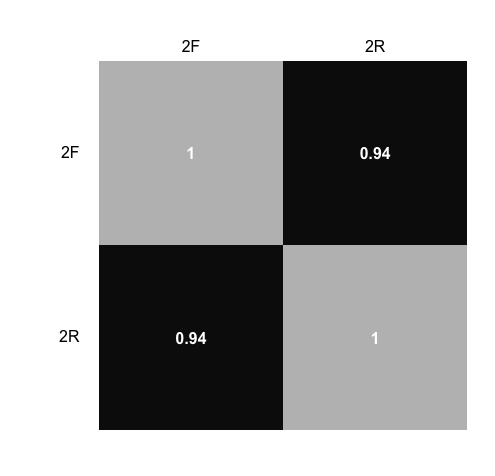
\includegraphics[width=\linewidth]{cor_mkt41}
  \caption{Market 1}
  \label{fig:cor_mkt4}
\end{subfigure}%
\begin{subfigure}{.5\textwidth}
  \centering
  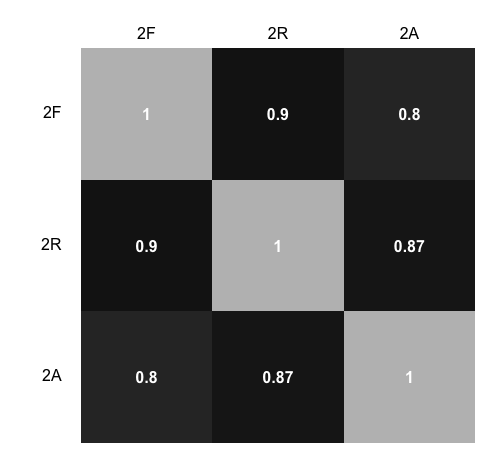
\includegraphics[width=\linewidth]{cor_mkt21}
  \caption{Market 2}
  \label{fig:cor_mkt2}
\end{subfigure}%

\begin{subfigure}{.5\textwidth}
  \centering
  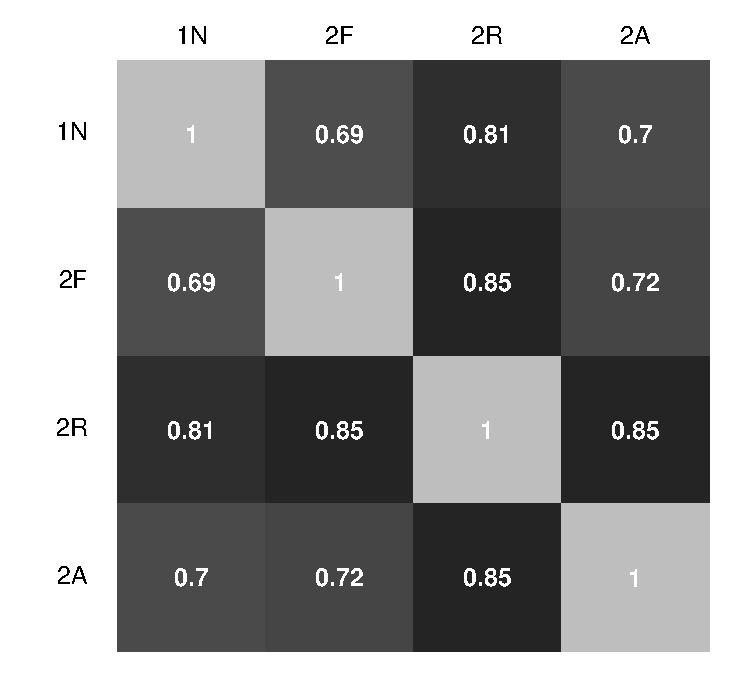
\includegraphics[width=\linewidth]{cor_mkt3_SCOTYORK}
  \caption{Market 3}
  \label{fig:cor_mkt3}
  \end{subfigure}%
\begin{subfigure}{.5\textwidth}
  \centering
  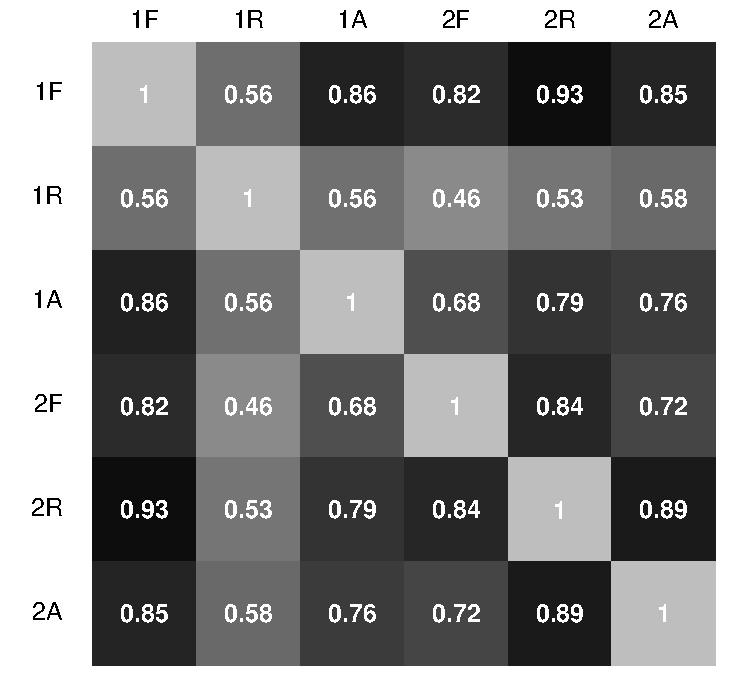
\includegraphics[width=\linewidth]{cor_mkt4_SCOTYORK}
  \caption{Market 4}
  \label{fig:cor_mkt1}
\end{subfigure}%
\caption{Correlation of fares by market}
\label{fig:cor}
\caption*{Source: Own work}
\end{figure}

In Market 1, there is a high correlation between fares, computed as $0.94$. Also for the Market 2 the correlations are still very high, above of $0.80$. For Market 3, correlation assumes lower values, but still for the \textit{reduced} and \textit{advance}, and \textit{reduced} and \textit{full} tickets of the standard class they are very high, deemed as $0.85$ for both. For Market 4, correlations above $0.80$ for two-fifths of the coefficients.

Despite the presence of high correlation among the fares, it should not be an issue in Bayesian regression when strong informative priors are provided, as discussed in Chapter \ref{chp:lit-rev}. 

 % Despite the bayesian approach does not overcomer this issue, it has a different way to deal with it, as discussed previously in Chapter \ref{chp:lit-rev}. It is important, therefore, to idenfity the extension of correlation in the data to be aware of it when stablishing the priors and interpreting the results. 

\section{Model}
% 400 words

Bayesian models are usually wrote formally as shown in Equation \ref{eq:model}. This format is useful to identify the elements that must conceptualised when building a model: the linear model, the likelihood, and the priors. Next subsections will work on these elements.

% In order to conceptualize a model, \cite{mcelreath2012} presents a useful framework especially for bayesian methods, even though it can be expanded for all kind of techniques. This scheme is a sequence of decision that helps to identify the elements of the model. Figure \ref{fig:model_decision_framework} illustrates it.

% \begin{figure}[H]
% \centering
% 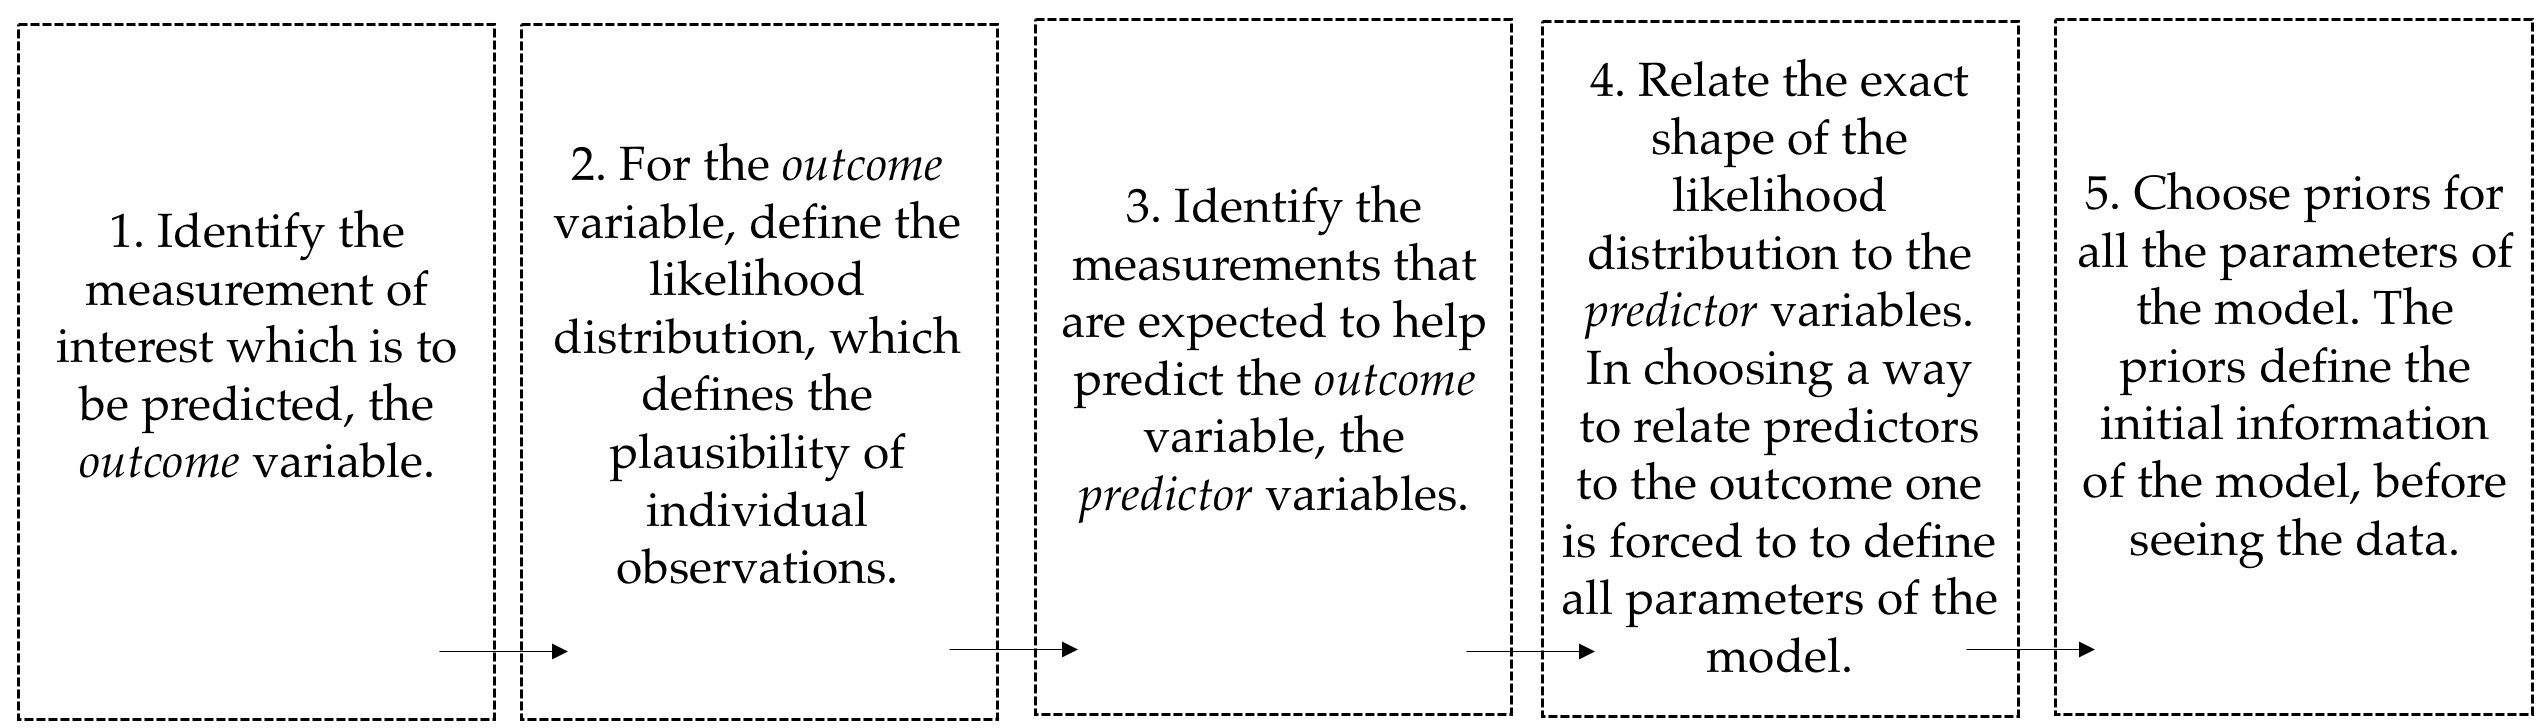
\includegraphics[width=\linewidth]{model_decision_framework}
% \caption{Generic framework to define a model}
% \label{fig:model_decision_framework}
% \caption*{Source: \cite{mcelreath2012}, p.77 [adapted]}
% \end{figure} 

% With these decisions made, the model can be stated, for example, in the format shown in Equation \ref{eq:model}. This format can be retrieved from the example given in Chapter \ref{chp:lit-rev}.

\begin{align}
\label{eq:model}
\text{outcome}_i \sim& Normal(\mu_i, \sigma) && \text{[likelihood]} \\
\mu_i =& \beta \times \text{predictor}_i     && \text{[linear model]}\nonumber\\
\beta \sim& Normal (\mu_\beta, \sigma_\beta) && \text{[prior]}\nonumber\\
\sigma \sim& uniform(a,b) \nonumber          && \text{[prior]}
\end{align}

%  The actual statement for the models are presented in the Appendix \ref{apd:model_statement}.

\subsection{Linear model}

The demand model adopted in this study is the one presented Equation \ref{eq:demand_pdfh}, Chapter \ref{chp:lit-rev}. 

% \begin{equation}
% \label{eq:demand_pdfh}
% V_{i} = a \; \text{GVA}^g_i \; P^f_i \; \text{GJT}^\gamma_i
% \end{equation}
% where

% $V_i$ is volume of journeys, the outcome variable;

% $a$ is a constant;

% $GVA_i$ is the gross added value, one of the predictor variables;

% $P_i$ is the price of the ticket, one of the predictor variables;

% $GJT_i$ is the generalised journey time, one of the predictor variables;

% $g$ is the GVA elasticity of demand;

% $f$ is the price elasticity of demand;

% $\gamma$ is the GJT elasticity of demand.
% \\[3pt]

A stochastic version of this model is given simply by adding the error term into Equation \ref{eq:demand_pdfh}, as shown by Equation \ref{eq:demand_pdfh_stoc}.

\begin{equation}
\label{eq:demand_pdfh_stoc}
V_{i} = a \; {GVA}^g_i \; P^f_i \; GJT^\gamma_i \; e^{u_i}
\end{equation}

A linear alternative to express exponential relationships is the double-log form, as shown by Equation \ref{eq:double_log}. The linear alternative is convenient because it allows estimation by linear regression models and the estimated coefficients can be interpreted as elasticities. %, which allows learning ``about the mean and variance of a measurement using an additive combination of others measures" \citep[p.~71]{mcelreath2012}.

\begin{equation}
\label{eq:double_log}
ln V_{i} = ln \; a + \; g \; ln {GVA}_i + f \; ln P_i + \gamma \; GJT_i + u_i
\end{equation}

Because the interest is to estimate price elasticities of each specific fares, the price component of the model and its elasticity will vary according to the range of available fares in the considered market. Therefore, for Market 1, the price component will be expanded to $f_{2F} ln P_{2F}$ and $f_{2R} ln P_{2R}$, for fares $2F$ and $2R$ respectively. Also, different systems of equations will be estimated for different markets according to the fares available. For instance, in Market 1, there will be two equations: one to estimate the demand of fare 2F and one to estimate the demand of fare 2R. Therefore, the generic form of the equations to be estimated will be, as shown by Equation \ref{eq:generic_model}.

\begin{equation}
\label{eq:generic_model}
ln V_{ki} = ln \; a + \; g \; ln {GVA}_i + \sum{f_{k} \; ln P_{ki}} + \gamma \; GJT_i + u_i
\end{equation}
where

$k$ is the available type of fares in the market.
\\[3pt]

For completeness, the relation of outcomes and predictor variables in each market is shown in the Appendix \ref{apd:linear_models}.

 % It worths highlight that each elasticity regards the demand estimated in its respective equation. Therefore, for market 1, for instance, the first equation will give estimates of fare elasticities $f_{2F}$ and $f_{2R}$ with respect to $V_{2F}$, and the second equation with respect to $V_{2R}$. This was omitted to avoid over subscription in the equations.

% \begin{landscape}
% 
% \begin{table}[!ht] \centering 
%   \caption{Estimated models by market} 
%   \label{tbl:equation_panel} 
% {\renewcommand\arraystretch{1.25}}
% \begin{tabular} {clll}
% \toprule
% Market            & Estimated Equations & Fares Elasticities\\
% \hline
% \multirow{2}{*}{1}&$V_{2Fi} = g{GVA}_i + f_{2F}P_{Fi} + f_{2R}P_{Fi} + \gamma GJT_i $ & $f_{2F}$ and $f_{2R}$, w.r.t. $V_{2F}$\\
%                   &$V_{2Ri} = g{GVA}_i + f_{2F}P_{Fi} + f_{2R}P_{Fi} + \gamma GJT_i $ & $f_{2F}$ and $f_{2R}$, w.r.t. $V_{2R}$\\


% \hline
% \multirow{3}{*}{2}&$V_{2Fi} = g{GVA}_i + f_{2F}P_{2Fi} + f_{2R}P_{Fi} + f_{2A}P_{2Ai} + \gamma GJT_i $ & $f_{2F}$, $f_{2R}$ and $f_{2A}$, w.r.t. $V_{2F}$\\
%                   & $V_{2Ri} = g{GVA}_i + f_{2F}P_{2Fi} + f_{2R}P_{2Ri} + f_{2A}P_{2Ai} + \gamma GJT_i $ & $f_{2F}$, $f_{2R}$ and $f_{2A}$, w.r.t. $V_{2R}$\\
%                   & $V_{2Ai} = g{GVA}_i + f_{2F}P_{2Fi} + f_{2R}P_{2Ri} + f_{2A}P_{2Ai} + \gamma GJT_i $ & $f_{2F}$, $f_{2R}$ and $f_{2A}$, w.r.t. $V_{2A}$\\
 

%  \hline
% \multirow{4}{*}{3}&$V_{1Ni} = g{GVA}_i + f_{1N}P_{1Ni} + f_{2F}P_{2Fi} + f_{2R}P_{2Ri} + f_{2A}P_{2Ai} + \gamma GJT_i $ & $f_{1N}$, $f_{2F}$, $f_{2R}$ and $f_{2A}$, w.r.t. $V_{1N}$\\
%                   &$V_{2Fi} = g{GVA}_i + f_{1N}P_{1Ni} + f_{2F}P_{2Fi} + f_{2R}P_{2Ri} + f_{2A}P_{2Ai} + \gamma GJT_i $ & $f_{1N}$, $f_{2F}$, $f_{2R}$ and $f_{2A}$, w.r.t. $V_{2F}$\\
%                   &$V_{2Ri} = g{GVA}_i + f_{1N}P_{1Ni} + f_{2F}P_{2Fi} + f_{2R}P_{2Ri} + f_{2A}P_{2Ai} + \gamma GJT_i $ & $f_{1N}$, $f_{2F}$, $f_{2R}$ and $f_{2A}$, w.r.t. $V_{2R}$\\
%                   &$V_{2Ai} = g{GVA}_i + f_{1N}P_{1Ni} + f_{2F}P_{2Fi} + f_{2R}P_{2Ri} + f_{2A}P_{2Ai} + \gamma GJT_i $ & $f_{1N}$, $f_{2F}$, $f_{2R}$ and $f_{2A}$, w.r.t. $V_{2A}$\\
 

%  \hline
% \multirow{6}{*}{4}&$V_{1Fi} = g{GVA}_i + f_{1F}P_{1Fi} + f_{1R}P_{1Ri} + f_{1A}P_{1Ai} + f_{2F}P_{2Fi} + f_{2R}P_{2Ri} + f_{2A}P_{2Ai} + \gamma GJT_i $ & $f_{1N}$, $f_{2F}$, $f_{2R}$ and $f_{2A}$, w.r.t. $V_{1F}$\\
%                   &$V_{1Ri} = g{GVA}_i + f_{1F}P_{1Fi} + f_{1R}P_{1Ri} + f_{1A}P_{1Ai} + f_{2F}P_{2Fi} + f_{2R}P_{2Ri} + f_{2A}P_{2Ai} + \gamma GJT_i $ & $f_{1N}$, $f_{2F}$, $f_{2R}$ and $f_{2A}$, w.r.t. $V_{1R}$\\
%                   &$V_{1Ai} = g{GVA}_i + f_{1F}P_{1Fi} + f_{1R}P_{1Ri} + f_{1A}P_{1Ai} + f_{2F}P_{2Fi} + f_{2R}P_{2Ri} + f_{2A}P_{2Ai} + \gamma GJT_i $ & $f_{1N}$, $f_{2F}$, $f_{2R}$ and $f_{2A}$, w.r.t. $V_{1A}$\\
%                   &$V_{2Fi} = g{GVA}_i + f_{1F}P_{1Fi} + f_{1R}P_{1Ri} + f_{1A}P_{1Ai} + f_{2F}P_{2Fi} + f_{2R}P_{2Ri} + f_{2A}P_{2Ai} + \gamma GJT_i $ & $f_{1N}$, $f_{2F}$, $f_{2R}$ and $f_{2A}$, w.r.t. $V_{2F}$\\
%                   &$V_{2Ri} = g{GVA}_i + f_{1F}P_{1Fi} + f_{1R}P_{1Ri} + f_{1A}P_{1Ai} + f_{2F}P_{2Fi} + f_{2R}P_{2Ri} + f_{2A}P_{2Ai} + \gamma GJT_i $ & $f_{1N}$, $f_{2F}$, $f_{2R}$ and $f_{2A}$, w.r.t. $V_{2R}$\\
%                   &$V_{2Ai} = g{GVA}_i + f_{1F}P_{1Fi} + f_{1R}P_{1Ri} + f_{1A}P_{1Ai} + f_{2F}P_{2Fi} + f_{2R}P_{2Ri} + f_{2A}P_{2Ai} + \gamma GJT_i $ & $f_{1N}$, $f_{2F}$, $f_{2R}$ and $f_{2A}$, w.r.t. $V_{2A}$\\
% \bottomrule\end{tabular}%
% \caption*{Source: own elaboration}
% \end{table} 


\begin{table} \centering 
  \caption{Linear models by market} 
  \label{tbl:equation_panel} 
{\renewcommand\arraystretch{1.25}}
\begin{tabular} {cl}
\toprule
Market            & Equations \\
\hline
\multirow{2}{*}{1}&$lnV_{2Fi} = ln \; a + g \; ln{GVA}_i + f_{2F} \; lnP_{2Fi} + f_{2R} \; lnP_{2Ri} + \gamma \; lnGJT_i$ \\
                  &$lnV_{2Ri} = ln \; a + g \; ln{GVA}_i + f_{2F} \; lnP_{2Fi} + f_{2R} \; lnP_{2Ri} + \gamma \; lnGJT_i$ \\


\hline
\multirow{3}{*}{2}&$lnV_{2Fi} = ln \; a + g \; ln{GVA}_i + f_{2F} \; lnP_{2Fi} + f_{2R} \; lnP_{2Ri} + f_{2A} \; lnP_{2Ai} + \gamma \; lnGJT_i$\\
                  &$lnV_{2Ri} = ln \; a + g \; ln{GVA}_i + f_{2F} \; lnP_{2Fi} + f_{2R} \; lnP_{2Ri} + f_{2A} \; lnP_{2Ai} + \gamma \; lnGJT_i$\\
                  &$lnV_{2Ai} = ln \; a + g \; ln{GVA}_i + f_{2F} \; lnP_{2Fi} + f_{2R} \; lnP_{2Ri} + f_{2A} \; lnP_{2Ai} + \gamma \; lnGJT_i$\\
 

 \hline
\multirow{4}{*}{3}&$lnV_{1Ni} = ln \; a + g \; ln{GVA}_i + f_{1N} \; lnP_{1Ni} + f_{2F} \; lnP_{2Fi} + f_{2R} \; lnP_{2Ri} + f_{2A} \; lnP_{2Ai} + \gamma \; lnGJT_i$\\
                  &$lnV_{2Fi} = ln \; a + g \; ln{GVA}_i + f_{1N} \; lnP_{1Ni} + f_{2F} \; lnP_{2Fi} + f_{2R} \; lnP_{2Ri} + f_{2A} \; lnP_{2Ai} + \gamma \; lnGJT_i$\\
                  &$lnV_{2Ri} = ln \; a + g \; ln{GVA}_i + f_{1N} \; lnP_{1Ni} + f_{2F} \; lnP_{2Fi} + f_{2R} \; lnP_{2Ri} + f_{2A} \; lnP_{2Ai} + \gamma \; lnGJT_i$\\
                  &$lnV_{2Ai} = ln \; a + g \; ln{GVA}_i + f_{1N} \; lnP_{1Ni} + f_{2F} \; lnP_{2Fi} + f_{2R} \; lnP_{2Ri} + f_{2A} \; lnP_{2Ai} + \gamma \; lnGJT_i$\\ 
 \hline
\multirow{6}{*}{4}&$lnV_{1Fi} = ln \; a + g \; ln{GVA}_i + f_{1F} \; lnP_{1Fi} + f_{1R} \; lnP_{1Ri} + f_{1A} \; lnP_{1Ai} + f_{2F} \; lnP_{2Fi} + f_{2R} \; lnP_{2Ri} + f_{2A} \; lnP_{2Ai} + \gamma \; lnGJT_i$\\
				  &$lnV_{1Ri} = ln \; a + g \; ln{GVA}_i + f_{1F} \; lnP_{1Fi} + f_{1R} \; lnP_{1Ri} + f_{1A} \; lnP_{1Ai} + f_{2F} \; lnP_{2Fi} + f_{2R} \; lnP_{2Ri} + f_{2A} \; lnP_{2Ai} + \gamma \; lnGJT_i$\\
				  &$lnV_{1Ai} = ln \; a + g \; ln{GVA}_i + f_{1F} \; lnP_{1Fi} + f_{1R} \; lnP_{1Ri} + f_{1A} \; lnP_{1Ai} + f_{2F} \; lnP_{2Fi} + f_{2R} \; lnP_{2Ri} + f_{2A} \; lnP_{2Ai} + \gamma \; lnGJT_i$\\
				  &$lnV_{2Fi} = ln \; a + g \; ln{GVA}_i + f_{1F} \; lnP_{1Fi} + f_{1R} \; lnP_{1Ri} + f_{1A} \; lnP_{1Ai} + f_{2F} \; lnP_{2Fi} + f_{2R} \; lnP_{2Ri} + f_{2A} \; lnP_{2Ai} + \gamma \; lnGJT_i$\\
				  &$lnV_{2Ri} = ln \; a + g \; ln{GVA}_i + f_{1F} \; lnP_{1Fi} + f_{1R} \; lnP_{1Ri} + f_{1A} \; lnP_{1Ai} + f_{2F} \; lnP_{2Fi} + f_{2R} \; lnP_{2Ri} + f_{2A} \; lnP_{2Ai} + \gamma \; lnGJT_i$\\
				  &$lnV_{2Ai} = ln \; a + g \; ln{GVA}_i + f_{1F} \; lnP_{1Fi} + f_{1R} \; lnP_{1Ri} + f_{1A} \; lnP_{1Ai} + f_{2F} \; lnP_{2Fi} + f_{2R} \; lnP_{2Ri} + f_{2A} \; lnP_{2Ai} + \gamma \; lnGJT_i$\\

\bottomrule\end{tabular}%
\caption*{Source: Own work}
\end{table} 

% \end{landscape}

\subsection{Likelihood}
% 300 words

The first thing to consider to define the likelihood is the scale type of the outcome variable - whether metric, ordinal, nominal or count. Because things can be measured in different scales, different probability measure may apply and ``the likelihood function must specify a probability distribution on the appropriate scale" \citep[p.~423]{kruschke2014}.

For this study, the outcome variable - \textit{journeys} - can be considered as metric scale, since its value actually provides a quantity of what is being measured - even though it is transformed to logarithmic form. 

For this kind of scale, the most usual probability distribution is the normal. \cite{mcelreath2012} discuss two main reasons that can justify it.

The first one regards the fact the normal distribution has the property to represent phenomenons that are sum of fluctuations of other phenomenons, irrespective of their original distribution. ``Repeatedly adding finite fluctuations results in a distribution of sums that shed all information about the underlying process, aside from mean and spread" \citep[p.~75]{mcelreath2012}. In this sense, it might be plausible to interpret the number of rail journeys as a resultant phenomenon of fluctuations of the subprocess. People often make travel decision based on a general range of factors, and the way they usually vary in time and region may represent the fluctuations mentioned.

The second reason regards the fact that the normal distribution ``represents a particular state of ignorance" \citep[p.~75]{mcelreath2012}. This represents the most convenient form to express the lack of knowledge about a variable because its shape can comprise several different assumptions.

This also seems to be applicable to our variable. Putting in another way, one may not have evidence that this should not assume a normal distribution and this ignorance may suggest normal it is appropriate.

Therefore, the likelihood which will be applied for all models will be such as $ln V_i \sim Normal(\mu_i, \sigma)$.

\subsection{Priors} 

When defining a prior distribution, one must be aware of two aspects of it: first it regards the definition of an interval for credible values that the parameter can assume; second, regards the shape of the probability density in this interval. To consider these elements for the current case, one may first recover the parameters presented in Equation \ref{eq:demand_pdfh}, summarised by Table \ref{tbl:param_priors}.


\begin{table}[!ht] \centering 
  \caption{Model's parameters that demand prior distributions} 
  \label{tbl:param_priors} 
{\renewcommand\arraystretch{1.25}}
\begin{tabular} {clc}
\toprule
\multirow{2}{*}{Parameter}  & \multirow{2}{*}{Measure}  & Expected \\
                            &                           & Sign \\
\hline
\multirow{2}{*}{$f$}        & price elasticity of demand.& own: negative \\
		   & It can regard the own or cross elasticity.  & cross: positive\\
$g$        & GVA elasticity of demand. & positive \\ 
$\gamma$   & GJT elasticity of demand. & negative\\
$\sigma$   & standard deviation of the outcome variable.& N.A.\\
\bottomrule
\end{tabular}%
\caption*{Source: Own work}
\end{table} 



Starting for the price elasticity, it will be convenient divide it in two discussions: the own elasticity prior and the cross elasticity prior. This is relevant because of the assumption adopted from the PDFH that the differently available fares are competitors, thus the cross elasticity should expect to be positive, and the own elasticity should expect to be negative. 

Recovering that the price elasticity measures how much the demand responds to a change in price, in percentage terms, one may consider plausible that credible values for the own price elasticities of demand in this study should be somewhere between zero and -1. This interval covers circumstances which go from a complete inelastic demand, which does not vary irrespective of a change in price, to an elastic demand, in which case a change in price causes a proportional change in the demand in the opposite direction. It eventually could be lower than -1, for a very price-sensitive demand, but it would not be reasonable considering that there is no lower boundary, even though setting one may be arbitrary.

For the cross elasticity, the rationale is analogous but the values are symmetric, so a credible interval would be between zero and 1. Again, it would eventually be greater than 1, even though it may be arbitrary setting an upper boundary. 

% IS IT POSSIBLE TO DISCUSS THAT THE CROSS ELASTICITIES ARE SMALLER THAN THE OWN ELASTICITIES?
% To complement this analysis, it should be also considered that cross-elasticities should be expected to be smaller that the own elasticities of demand. Cross-elasticity, opposed to the own-elasticity, regards a marginal effect of a change in the price of a secondary good. For instance, when a price of good B increases, its own demand may be reduced because consumers stop to consume it or because they migrate to competitive  it may reflect the demand of 

In what regards the shape of the probability density across the credible values for price elasticities, economic theory provides no evidence abaout it, which may lead to the adoption of a uniform probability. However, the guidances from the statistical package used in this work - Stan \citep{stan}, suggests as a general principle that uniform priors should not be applied ``unless the boundaries represent true constraints" \citep{stan_prior}. Despite one of the boundaries actually represent a constraint - the upper boundary is zero for own elasticity and the lower boundary is also to zero for the cross elasticity - the others boundaries would be defined arbitrarily. Therefore, adopting uniform distribution would be not a goodd practice. 

The suggested solution is to stablish a normal distribution centred in the credible interval. Indeed, there are specific guidances for elasticities estimates in double-log regressions that recommends that normal distribution with mean $0.5$ and standard deviation of $0.5$ is a good default prior.

To ensure that the theoretical constraints will be respected, a one-sided restriction will be applied, as pertinent. As introduced in Chapter \ref{chp:lit-rev}, the possibility of applying constraints is one of the advantages of Bayesian inference. 

For own price elasticities, the prior will be defined as $f \sim Normal(-0.5, 0.5)$, truncated at zero at the upper boundary ($T[ \quad , 0]$); and for cross price elasticities, $f_x \sim Normal(0.5, 0.5)$, trucated at zero at the lower bound ($T[0, \quad]$).

For the GVA elasticity of demand, the prior knowledge suggests a positive polarity between the rail demand and the GVA, as already discussed in the exploratory analysis of the data in this Chapter. Even though the GVA elasticity is expected to be positive, this single piece of information is not enough to define the interval for credible values and the shape of probability density function. It will be convenient, thus, follow the guidances from the statistical package - Stan. A suggested generic prior is recommended to be Normal(0,1). The guidance highlights that this prior may limit extreme values because the normal distribution has shorter tails than other bell-shaped distributions. 

The GJT elasticity of demand is analogous to the GVA but in the opposite direction. As discussed in the exploratory analysis, an increase in GJT tends to cause decrease in the demand, so a negative coefficient should be expected. For the same reasons presented for the GVA elasticity, it will also be adopted the generic prior Normal(0,1) to the GJT parameter.

Lastly, as done for the price elasticity priors, to ensure right algebraic signs, the prior distribution for GVA and GJT elasticities will be constrained by a lower and upper boundary at zero, respectively. 

% Lastly, despite being possible to restrict the values to be positive or negative for both GVA and GJT parameters, as was done in the price elasticity priors, it would not be done to avoid unnecessary constraints in the model. Unless it became necessary to correct the algebraic sign of the estimate, they will not be restricted.

Therefore, for the GVA and the GJT's elasticities the prior applied will be $g \sim Normal(0,1)$, truncated at zero at the lower boundary ($T[0, \quad ]$) and $\gamma \sim Normal(0,1)$, truncated at zero at the upper boundary ($T[ \quad , 0]$), respectively. 

For the $\sigma$ prior there is no evident definition for a range of credible values, despite the fact that it is by nature a positive value. It was adopted the default distribution from Stan - uniform prior on ($-\infty$, $\infty$) \citep{stan-manual} - constrained by the positive domain. Therefore, the resulting $\sigma$'s prior was $\sigma \sim uniform(0,\infty)$.

% The whole model is presented in the Appendix \ref{apd:model_statement}. 

% \textit{Prior Sensitivness}

\section{Calibration and target measures}

As mentioned, the Bayesian models were estimated with the aid of the \textit{Stan}, a software package. In this package the posterior distributions are approximated using a Markov Chain of Monte Carlo called \textit{Hamiltonia Monte Carlo}, a variation of the Metropolis algorithm.

Some elements of the estimation process that are important to interpret the results regard the calibration of the process in terms of number of iterations, warm-up period, thinness, number of chains, initial values, effective sample and autocorrelation measures, and convergence. A brief definition and the default adopted in this work are presented in the following.

The quantity of iterations regards the length of the Markov Chain that will be run to build the posterior distribution. The longer it is, the more defined the posterior gets. However, it does not mean that one needs to exhaust computation resources to get a reasonable draw of posterior distributions. For this work, the standard number of iterations adopted was $2,000$. It is supposed to be enough to achieve convergence without autocorrelated samples, for non-complex models. Eventually, more iterations may be demanded.

Still regarding the number of iterations, is the warm-up period, which is ``the practice of discarding early iterations in Markov Chain (...) to diminish the influence of starting values" \citep{gelman2014}. The discarded ratio may vary according to the circumstances, but for a conservative approach, it will be adopted to discard the first half of the iterations. Therefore, running $2,000$ iterations, the first $1,000$ will be discarded.

Another aspect of the Markov Chain regards thinness of steps, which is the rule of which steps are kept as a draw for the posterior. It is usually defined as 1, so each iteration is kept. Nevertheless, it may be increased to reduce autocorrelation \citep{kruschke2011} - instead of keeping each iteration, one keeps only every $n^{th}$ step. An implication of increasing the thinness of an estimation is that it reduces the iterations kept, which might demand as a counterpart the increase of the number of iterations proportionally. In this study it will be adopted thin = 1. If it eventually demands to be increased to $n$, the interactions will be $2,000 \cdot n$.

Despite defining the number of iterations and its related attributes, it is also necessary to define the number of chains. After the warm-up period the variance within the chain is supposed to be stable, so one may consider that it has achieved convergence. However, for a reliable inference, it is also important to check whether different independent sequences will converge to the same distribution. In this study, it will be adopted the default of 3 chains. When discussing the results a measure for convergence will be the $\hat{R}$, the potential scale reduction factor. When convergence is achieved, $\hat{R}=1$.

Another element that needs to be calibrated in the estimation procedure is the initial values from which the Markov Chains will start. For this study the default will not be explicitly defined. Instead, they will be randomly generated by the software \citep{stan-manual}.

Lastly, there is the the effective sample size ($n_{\text{eff}}$), which is not an element to be calibrated in the process but an output used to judge the quality of the resulting posterior distribution in combination with the $\hat{R}$. As long it will be used in Chapter \ref{chp:results}, it worths introducing its concept. 

When samples are autocorrelated in the chain the estimation might become inefficient because it does not fully explore the probability space of the parameters, instead it may get stuck. The $n_{\text{eff}}$ is a measure that discount autocorrelated samples, providing a sense of the number of independent samples drawn to estimate the posterior distribution. As a default rule, \cite{gelman2014} suggests running the simulation until $n_{eff}$ is at least ten times the number of chains. Therefore, since the estimation will run with 3 chains, the $n_{\text{eff}}$ must be higher than 30.